\documentclass[pdflatex,sn-mathphys-num]{sn-jnl}
\usepackage[T1]{fontenc}\usepackage[utf8]{inputenc}\usepackage{lmodern}
\usepackage{microtype}
\usepackage{amsmath,amssymb,amsfonts,amsthm,mathtools}
\usepackage{graphicx,booktabs,array,multirow,enumitem,tabularx,longtable}
\usepackage{xcolor,siunitx,listings}
\usepackage{threeparttable}
\usepackage{tikz}
\usetikzlibrary{shapes.multipart, calc, positioning, backgrounds, shadows, arrows.meta, fit}
\usepackage{float}       % For [H] placement
\usepackage{caption}     % For caption formatting

% Color palette for the architecture figure
\definecolor{layerbg}{RGB}{248, 249, 250}
\definecolor{layerborder}{RGB}{173, 181, 189}
\definecolor{headerbg}{RGB}{233, 236, 239}
\definecolor{headertext}{RGB}{33, 37, 41}
\definecolor{codetext}{RGB}{0, 86, 179}
\definecolor{arrowcolor}{RGB}{108, 117, 125}

\emergencystretch=2em

\lstset{basicstyle=\ttfamily\small,breaklines=true,frame=single,
        columns=fullflexible,backgroundcolor=\color{gray!6}}

\DeclareMathOperator{\Tr}{Tr}\DeclareMathOperator{\rank}{rank}
\newcommand{\cD}{\mathcal{D}}\newcommand{\cH}{\mathcal{H}}
\newcommand{\cN}{\mathcal{N}}\newcommand{\cR}{\mathcal{R}}
\newcommand{\cU}{\mathcal{U}}
\newcommand{\cC}{\mathcal{C}}
\newcommand{\norm}[1]{\left\lVert #1\right\rVert}
\newcommand{\ket}[1]{\lvert #1\rangle}
\newcommand{\proj}[1]{\lvert #1\rangle\!\langle #1\rvert}

\theoremstyle{thmstyleone}
\newtheorem{theorem}{Theorem}
\newtheorem{proposition}[theorem]{Proposition}
\newtheorem{lemma}[theorem]{Lemma}
\newtheorem{corollary}[theorem]{Corollary}
\theoremstyle{thmstyletwo}
\newtheorem{remark}{Remark}
\theoremstyle{thmstylethree}
\newtheorem{definition}{Definition}

\begin{document}
\title[Decoder Evaluation and Risk Certification]{Decoder Evaluation and Adversarial-Risk Certification for Quantum Error-Correcting Memories}
\author[1]{\fnm{Saleh H.} \sur{AlDaajeh}}
\author[2]{\fnm{Saud} \sur{Aldajah}}\email{Saud.Aldajah@sma.ac.ae}
\author[3*]{\fnm{Sadi} \sur{Alawadi}}\email{sadialawadi@uaeu.ac.ae}
\author[4]{\fnm{Mohammad} \sur{Hayajneh}}
\author[5]{\fnm{Wesam} \sur{Almobaideen}}
\author[6,7]{\fnm{Ja'far} \sur{Alqatawna}}\email{Jalqatawna@hct.ac.ae}
\affil[1]{\orgdiv{Department of Computing Sciences}, \orgname{Rochester Institute of Technology}, \country{UAE}}
\affil[2]{\orgname{Sharjah Maritime Academy}, \country{UAE}}
\affil[3]{\orgdiv{Statistics and Business Analytics}, \orgname{United Arab Emirates University}, \city{Al Ain}, \country{UAE}}
\affil[4]{\orgdiv{Department of Computer Networks Engineering}, \orgname{United Arab Emirates University}, \country{UAE}}
\affil[5]{\orgdiv{Department of Computing Sciences}, \orgname{Rochester Institute of Technology}, \country{UAE}}
\affil[6]{\orgdiv{Faculty of Computer Information Science}, \orgname{Higher Colleges of Technology}, \country{UAE}}
\affil[7]{\orgdiv{King Abdullah II School for Information Technology}, \orgname{The University of Jordan}, \country{Jordan}}

\abstract{Reliability claims for quantum error-correcting memories are only as strong as the evidence behind them, yet decoder benchmarks are rarely pinned to an explicit implementation, noise representation, and failure endpoint, and worst-case fault tolerance is rarely measured at all. We present an evidence-graded framework that evaluates decoder performance and bounded adversarial-fault risk together. For a fixed code, schedule, decoder, and native-noise model we define the operational risk $\lambda_{\mathcal{M}}(W)=\max_{|F|\le W}\Pr[\text{logical failure}\mid F]$, decompose outcomes through a four-category endpoint that separates logical failures from invalid decoder outputs and aborts, and report Bonferroni-simultaneous intervals with at least 95\% joint coverage within each stated family; where tested attacks do not exhaust the weight budget we report $U_W=1$ unless an analytic bound covers the untested region. We prove a spacetime-budget correctability theorem with an explicit sharpness construction for repetition memories, a device-aware composition bound, a CSS extension under stated decoding assumptions, and a Pauli-channel relation between sector-wise logical failure and diamond distance whose coherent residual we close analytically for REP3; minimax and Knill--Laflamme results are cited as background. For the pinned BB72 instance, exhaustive verification certifies $d=6$ and correction of every error of weight at most two under the specified decoder. Under code-capacity noise, BP+OSD outperforms the submitted DEM-chain matching and UF-BFS graphifications across BB72, BB144, and BB288, with risk ratios refined by a $10^{6}$-trial campaign to a joint-confidence lower bound above $134{,}000\times$ for BB288; on a 70{,}000-instance paired BB72 grid, BP-augmented configurations lie within a reported $\pm0.5$ percentage-point margin of BP+OSD, a descriptive comparison whose margin was fixed after the initial grid. Extending the repeated-cycle ladder upward in error rate resolves two successive, mutually consistent curve crossings, bracketed at $p_{\times}\in(0.036,0.040)$ ($d{=}6/12$) and $(0.032,0.036)$ ($d{=}12/18$), with the suppression factor collapsing as $\Lambda=3.46\to1.09$. The rungs are not equally resolved: the first crossing is interval-separated at both bracket endpoints, whereas the second is interval-separated at its lower endpoint and rests on a point-estimate inversion with overlapping intervals at its upper endpoint, and deep sub-threshold BB144-to-BB288 ratios remain unresolved at the achieved sample sizes. We therefore report graded finite-size crossing evidence under a pinned phenomenological protocol, not an asymptotic threshold estimate. On hardware, pre-registered injection campaigns on ibm\_marrakesh and ibm\_fez reproduce the predicted correctability boundary across distances $3$, $5$, and $7$, two calibration cycles, and two devices, and an executed causal ablation (160{,}000 shots) bounds the idle-decoherence contribution below $4\times10^{-4}$, finds calibration-informed placement directionally consistent but sub-threshold ($p=0.058$ against a pre-registered $\alpha=0.01$), and tightens the widest archived stochastic interval by $55\%$. The device experiments use repetition-code memories and do not establish BB-code hardware performance. All data, code, seeds, and SHA-256 provenance are archived.}
\keywords{quantum error correction, quantum LDPC codes, decoder benchmarking, adversarial risk, BP+OSD, matching decoders, finite-size scaling, hardware validation}
\maketitle
\noindent\textbf{Archive and emulator:} reproduction archive at Zenodo (concept DOI 10.5281/zenodo.20588042, always resolves to the latest version); QEC Emulator v2.0.0~\cite{AlDaajeh2026emulator} (ldpc 2.4.1, pymatching 2.2.2, stim 1.16.0, numpy 2.5.2).

%%-----------------------------------------------------------
\section{Introduction}
%%-----------------------------------------------------------

Quantum error correction turns a collection of noisy physical qubits into a reliable logical memory, and the reliability of that memory is an empirical quantity: it depends on the code, the noise the device actually produces, and the decoder that interprets the syndrome. Quantum low-density parity-check (qLDPC) codes have moved this interplay to the center of the field, because they combine bounded-weight checks with nonzero encoding rates and are now candidates for near-term fault-tolerant architectures. Bivariate-bicycle (BB) codes are the most prominent finite-size family, with weight-six stabilizers and competitive reported performance~\cite{Bravyi2024}. Assessing such memories responsibly requires more than quoting a single average logical-error rate: every claim must be tied to the implementation, the noise representation, and the evidence that supports it.

Decoder comparisons are particularly sensitive to representation. BB checks induce weight-three and higher detector structures, whereas standard graph-based matching expects pairwise edges, so any matching-based evaluation must first reduce the hypergraph---and a lossy reduction can conflate the decoder's performance with the preprocessor's. A meaningful comparison therefore pins both the algorithm and its input representation, uses matched noise instances where conclusions are comparative, and retains enough provenance for an independent auditor to replay the analysis end to end.

This paper pursues two related but deliberately distinct aims. The first is formal: we define the operational adversarial risk $\lambda_{\mathcal{M}}(W)$ of a fixed implementation as the worst-case logical-failure probability over injected fault sets of weight at most $W$, and we develop the surrounding theory---correctability with a matching sharpness construction, composition with native device noise, a CSS extension, and a bridge from sector-wise failure rates to diamond distance (Definition~\ref{def:acevalue}; Theorem~\ref{thm:spacetime}; Corollaries~\ref{cor:css}, \ref{cor:stoch}; Proposition~\ref{prop:bridge}). A four-category endpoint separates logical failures from invalid decoder outputs and aborts, so that a decoder which declines to answer is never mistaken for a correct one (Definition~\ref{def:endpoint}). The second aim is empirical: we benchmark established message-passing, matching, and BP-augmented decoders under pinned code-capacity, repeated-cycle, and circuit-level protocols, and we take the theory layer to hardware through pre-registered injection campaigns. The decoder contribution is evaluative rather than synthetic: we assess existing algorithms and representations, and the minimax saddle point and Knill--Laflamme fidelity floor used for context are standard results, not contributions of this work.

The evidence is layered by scope, and the layering is part of the method. Exact finite-instance facts come first: for the pinned BB72 matrices, exhaustive verification certifies distance $d=6$ and correction of every weight-at-most-two error under the specified decoder. Controlled simulations then quantify decoder behavior across BB72, BB144, and BB288, including a repeated-cycle distance ladder whose upward extension resolves two successive curve crossings, bracketed at $p_{\times}\in(0.036,0.040)$ ($d{=}6/12$) and $(0.032,0.036)$ ($d{=}12/18$) under one pinned phenomenological protocol. Finally, three pre-registered hardware campaigns on ibm\_marrakesh and ibm\_fez test the injection-budget bound on repetition-code memories, replicate it across calibration cycles and devices, and convert the two principal simulation confounders---idle decoherence and qubit placement---into experimentally controlled device claims. Each layer is reported with its own uncertainty model, and no layer is asked to carry claims it cannot support: the hardware campaigns, in particular, concern repetition memories and do not establish BB-code hardware performance.

\subsection{Contributions}

\begin{enumerate}[leftmargin=1.6em,label=(\roman*)]
  \item \textbf{An operational adversarial-risk estimand.} We define $\lambda_{\mathcal{M}}(W)$ for a fixed implementation and report simultaneous intervals that distinguish tested evidence from incomplete attack coverage, with decoder-invalid outputs tracked separately from logical failures (Definitions~\ref{def:acevalue}, \ref{def:endpoint}; Remark~\ref{rem:intervals}).
  \item \textbf{Correctability and composition theory.} We prove a spacetime-budget correctability theorem with a matching sharpness construction, derive a device-aware composition bound, extend the analysis to CSS memories under explicit decoding assumptions, and relate sector-wise logical error to diamond distance under a Pauli-channel assumption, with the coherent residual closed analytically for REP3 (Theorem~\ref{thm:spacetime}; Corollaries~\ref{cor:css}, \ref{cor:stoch}; Proposition~\ref{prop:bridge}; Remark~\ref{rem:twirl-num}).
  \item \textbf{A finite-instance code certificate.} For the pinned BB72 matrices, exhaustive verification establishes $d=6$ exactly and the stated weight-two correction property, with published witnesses and a self-contained independent checker (Section~\ref{sec:cert}).
  \item \textbf{Controlled decoder comparisons.} We compare BP+OSD with two submitted graphifications across three BB codes, refine the separation with a $10^{6}$-trial rare-event campaign, and evaluate seven decoder configurations on 70{,}000 paired BB72 instances, together with one synthetic circuit-level operating point and a re-analysis of the released Kunlun detector model (Sections~\ref{sec:benchmark}--\ref{sec:circuit}).
  \item \textbf{A measured finite-size crossing.} Extending the repeated-cycle ladder to higher physical error rates under an unchanged protocol resolves strict, interval-separated size ordering for $p\le0.032$, a suppression factor collapsing monotonically to unity ($\Lambda=3.46\to1.09$), and two successive curve crossings bracketing the crossover region $(0.032,0.040)$ (Section~\ref{ssec:fss}).
  \item \textbf{Device and model evidence.} Hardware-informed simulations isolate the parameters affecting the modeled CZ/MS comparison; three pre-pinned repetition-code campaigns test the correctability boundary on device, replicate it across calibration cycles and a second device, and execute a causal ablation of the two principal simulation confounders, bounding the idle-decoherence contribution below $4\times10^{-4}$ and tightening the widest archived stochastic interval by $55\%$ (Section~\ref{sec:causal}; Appendices~\ref{app:injection}--\ref{app:injection-repl}).
  \item \textbf{Reproducibility.} The open-source QEC Emulator and the accompanying archive provide pinned code instances, seeds, data, independent checkers, and SHA-256 provenance for every reported analysis.
\end{enumerate}

\noindent\textbf{Scope and limitations.}
The claims are deliberately bounded. We report a bracketed crossing region from two successive measured crossings rather than a threshold point estimate: the $d{=}12/18$ upper endpoint is point-inverted with overlapping intervals, no drift extrapolation is made from two rungs, and no asymptotic threshold is claimed for any code or decoder. The adversarial analysis is fixed-implementation and non-adaptive; it does not provide cryptographic security, authentication, device attestation, or composability guarantees. The hardware-noise ablation study is a sensitivity analysis inside a simulation model, and its causal conversion is the executed campaign of Section~\ref{sec:causal}, whose pre-registered tests \emph{bound} the idle-decoherence and placement effects at the resolution of their shot budgets rather than establish them; those device claims cover one device, one calibration cycle, and distance-5 repetition memories.

%%-----------------------------------------------------------
\section{Related work}
%%-----------------------------------------------------------

Quantum LDPC constructions aim to combine nonzero rate with growing distance, and several algebraic families now support that program~\cite{TillichZemor2014,PanteleevKalachev2022,LeverrierZemor2022}. Bivariate-bicycle codes provide the finite-size platform for this work; their construction and decoding performance have been studied under stochastic noise, including networked variants~\cite{Bravyi2024,ShawRengaswamy2026}, and system-level studies supply the overhead and fault-tolerance context in which such codes must ultimately be evaluated~\cite{Gottesman2014,FawziGrospellierLeverrier2018,ChristandlFawziGoswami2025}.

\noindent\textbf{Decoder methods.} BP+OSD is the standard reference for qLDPC decoding~\cite{Roffe2020,ldpcPackage}. Matching methods such as PyMatching and Sparse Blossom operate on graphlike detector models~\cite{Higgott2023,SparseBlossom2025}, while Stim provides efficient circuit-level sampling and detector-model extraction~\cite{Gidney2021}. Recent work has expanded the design space in two directions relevant here: low-latency belief propagation, through Relay-BP and its FPGA realization~\cite{Muller2025relay,Johnson2026relayfpga}, and structure-exploiting matching, through symmetry matching for BB codes~\cite{SahayBrown2026} and BP-informed matching hybrids~\cite{Higgott2023belief}. Because these methods differ as much in the representation they consume as in the inference they perform, the representation supplied to each decoder is itself an experimental variable, and we treat it as one throughout. The released Kunlun detector model enables an independent, reproducible decoder re-analysis on hardware-derived data~\cite{Wang2026kunlun}, and defect-aware placement and decoding have been validated experimentally~\cite{Bartlett2026defect}.

\noindent\textbf{Reliability evidence and closest prior art.} Existing reliability analyses address questions complementary to ours. Fail-fast methods accelerate the estimation of rare failures under a nominal stochastic noise law~\cite{beverland2025failfast}, whereas trapping-set analyses characterize the failure configurations of a decoder under stochastic detector models~\cite{Pacenti2026trapping}. Robust-recovery work optimizes the defender's recovery for a specified channel~\cite{kosut2008robust}, and coherent-error analyses characterize channel effects beyond Pauli models~\cite{huang2019coherent}. The $\Lambda$-based reporting convention provides a standard summary of below-threshold suppression~\cite{Acharya2024lambda}, and formal-verification work develops tools for checking quantum programs and protocols~\cite{RandPaykinZdancewic2018,Hietala2021,Bordg2021,Lewis2023}. Table~\ref{tab:priorart} positions the closest sources. Two distinctions deserve emphasis. First, fail-fast estimates nominal stochastic risk, whereas this work targets worst-case adversarial risk over fault-set placement; the two are complementary, and rare-event sampling could in principle accelerate estimation where the attack region is large. Second, trapping-set analysis and our injection study both examine failure structure, but differ in whether the fault configuration is sampled from a stochastic model or selected under an explicit adversarial weight budget.

\begin{table}[htbp]\centering\small
\caption{Closest prior art and differentiation. Scope abbreviations: nom.\ = nominal stochastic noise; adv.\ = adversarial placement.}
\label{tab:priorart}
\begin{tabular}{@{}p{0.20\columnwidth}p{0.30\columnwidth}p{0.44\columnwidth}@{}}
\toprule
source & contribution & relation to this work \\\midrule
Bravyi et al.\ \cite{Bravyi2024} & BB codes, thresholds, hardware memory & we reuse the code family; they do not treat adversarial injection \\
Roffe et al.\ \cite{Roffe2020} & BP+OSD decoder & our reference decoder; benchmarked, not introduced here \\
Sahay et al.\ \cite{SahayBrown2026} & symmetry matching for BB codes & pinned-comparator subject; bare form non-viable on this instance, BP-augmented tied with BP+OSD \\
M\"uller et al.\ \cite{Muller2025relay} & Relay-BP real-time BP & benchmarked; circuit-level outcome separates from the code-capacity tie \\
Beverland et al.\ \cite{beverland2025failfast} & fail-fast rare-event probing (nom.) & strongest comparison; accelerated nom.\ estimation vs our adv.\ worst-case bounds; complementary \\
Pacenti et al.\ \cite{Pacenti2026trapping} & DEM trapping sets & stochastic failure structure; no adversarial budget or endpoint decomposition \\
Kosut et al.\ \cite{kosut2008robust} & recovery optimization for a fixed channel & defender-side optimization; our $\lambda_{\mathcal{M}}(W)$ fixes the implementation \\
Huang et al.\ \cite{huang2019coherent} & coherent-error channel analysis & basis of our twirling residual, which we close analytically \\
Acharya et al.\ \cite{Acharya2024lambda} & below-threshold $\Lambda$ reporting & reporting standard we delimit our block-$\Lambda$ against (no matched protocol) \\
\bottomrule
\end{tabular}
\end{table}
Section~\ref{sec:comparator} provides the paired quantitative comparison with the tested decoder constructions.

%%-----------------------------------------------------------
\section{Experimental platform and reproducible workflow}
\label{sec:emulator}
%%-----------------------------------------------------------

All numerical benchmarks and noise-model simulations reported here use QEC Emulator v2.0.0~\cite{AlDaajeh2026emulator}, an open-source Python package released under the MIT licence at DOI 10.5281/zenodo.20574329 (June 2026); the hardware campaigns use IBM Quantum execution, with the emulator and archived analysis tools supporting circuit preparation, validation, and provenance. This section describes the emulator's architecture and pinned code instances, its noise and decoding models, the benchmark workflow and provenance layer, and the validation suite, and closes with the extension points used by follow-on work.

\subsection{Architecture and pinned code instances}

The emulator is organised as five independent layers (Figure~\ref{fig:emulator-arch}), each with a single scientific responsibility:

\begin{enumerate}[leftmargin=1.6em,label=\textbf{L\arabic*.}]
  \item \textbf{Code construction} (\texttt{codes.py}): BB code algebra over $\mathbb{F}_2$, SHA-256 matrix fingerprints.
  \item \textbf{Decoders} (\texttt{decoders.py}): LookupDecoder, BPOSDDecoder, MWPMDecoder; common abstract interface.
  \item \textbf{Noise models} (\texttt{noise.py}): four models from phenomenological to hardware noise-model simulation.
  \item \textbf{Benchmark runners} (\texttt{benchmark.py}): five runners covering all experimental protocols in this paper.
  \item \textbf{Provenance} (\texttt{provenance.py}): SHA-256 integrity seals, manifest export, QC checks.
\end{enumerate}

The layers are strictly decoupled: adding a decoder, noise model, or benchmark runner requires implementing a single interface and touches no other layer. The design thereby mirrors the experimental pipeline itself---pin a code, choose a noise model and decoder, run a benchmark, retain the provenance.

\begin{figure}[H]
    \centering

    % Use tikzpicture to draw the stacked boxes architecture
    \begin{tikzpicture}[
        % Define styles for the tikz elements
        layer/.style={
            draw=layerborder,
            line width=0.8pt,
            fill=layerbg,
            rounded corners=4pt,
            rectangle,
            align=left,
            text width=11cm,
            inner sep=0pt,
            outer sep=0pt,
},
        header/.style={
            fill=headerbg,
            text=headertext,
            font=\bfseries\sffamily,
            align=left,
            minimum width=11cm,
            inner xsep=10pt,
            inner ysep=4pt,
            rounded corners=4pt,
},
        content/.style={
            font=\small,
            inner xsep=10pt,
            inner ysep=5pt,
            align=left
}
    ]

        % Helper macro to define a layer
        % #1: Node name (e.g., L5)
        % #2: Placement relative to previous (e.g., below=of L4)
        % #3: Layer Header Text
        % #4: Layer Content Text
        \def\drawlayer#1#2#3#4{
            \node[layer, #2] (#1) {
                \begin{tikzpicture}[
                    every node/.style={inner sep=0pt, outer sep=0pt},
                    node distance=0pt
                    ]
                    \node[header, anchor=north] (hdr) at (0,0) {\strut #3};
                    \fill[headerbg] (hdr.south west) rectangle ([yshift=2pt]hdr.south east); % Fix bottom rounding
                    \draw[layerborder, line width=0.8pt] (hdr.south west) -- (hdr.south east);
                    \node[content, anchor=north west] (cnt) at ([yshift=-1pt]hdr.south west) {
                        \begin{minipage}{10.5cm}
                            #4
                        \end{minipage}
};
                    % Invisible strut to give consistent bottom padding
                    \node[anchor=north, minimum height=2pt] at (cnt.south) {};
                \end{tikzpicture}
};
}

        % L5: Provenance
        \drawlayer{L5}{}
            {L5. Provenance}
            {\raggedright
             \textcolor{codetext}{\texttt{ProvenanceRecord}}: SHA-256(code, decoder, $p$, seed, failures) \\
             \textcolor{codetext}{\texttt{ProvenanceLogger}}: CSV/JSON export, \textcolor{codetext}{\texttt{unresolved\_pairs()}} QC check
}

        % L4: Benchmark runners
        \drawlayer{L4}{below=0.1cm of L5}
            {L4. Benchmark runners}
            {\raggedright
             \textcolor{codetext}{\texttt{run\_sweep}} $\mid$ \textcolor{codetext}{\texttt{run\_repeated\_cycle}} $\mid$ \textcolor{codetext}{\texttt{run\_threshold\_scan}} \\
             \textcolor{codetext}{\texttt{run\_fixed\_weight}} $\mid$ \textcolor{codetext}{\texttt{run\_distance\_certificate}}
}

        % L3: Noise models
        \drawlayer{L3}{below=0.1cm of L4}
            {L3. Noise models}
            {\raggedright
             \textcolor{codetext}{\texttt{PhenomenologicalModel}} $\mid$ \textcolor{codetext}{\texttt{RepeatedCycleModel}} \\
             \textcolor{codetext}{\texttt{CircuitLevelModel}} $\mid$ \textcolor{codetext}{\texttt{HardwareModel(CZ|MS)}}
}

        % L2: Decoders
        \drawlayer{L2}{below=0.1cm of L3}
            {L2. Decoders}
            {\raggedright
             \textcolor{codetext}{\texttt{LookupDecoder}} $\mid$ \textcolor{codetext}{\texttt{BPOSDDecoder}} $\mid$ \textcolor{codetext}{\texttt{MWPMDecoder}} \\
             \textcolor{codetext}{\texttt{BaseDecoder}}: \textcolor{codetext}{\texttt{decode\_z(syn)}} $\to$ correction mask
}

        % L1: Code construction
        \drawlayer{L1}{below=0.1cm of L2}
            {L1. Code construction}
            {\raggedright
             \textcolor{codetext}{\texttt{BBCode(ell, m, a\_exp, b\_exp)}} $\to$ $H_X, H_Z$ + SHA-256 pins
}

    \end{tikzpicture}

    \vspace{0.5cm}
    \caption{Five-layer architecture of QEC Emulator v2.0.0. Each layer has a single scientific responsibility and is independently extensible.}
    \label{fig:emulator-arch}
\end{figure}

\noindent\textbf{Code construction.}
The \texttt{BBCode} dataclass constructs BB codes from generator-polynomial exponents over $\mathbb{F}_2[x,y]/(x^\ell-1,y^m-1)$. Three named constructors pin the three code instances used throughout this paper:

\begin{center}
\small
\begin{tabular}{@{}lllrrl@{}}
\toprule
Constructor & $(\ell,m)$ & Polynomials & $n$ & $k$ & $H_X$ SHA-256 prefix \\
\midrule
\texttt{BB72()}  & $(6,\,6)$   & $A=x^3+y+y^2$, $B=y^3+x+x^2$ & 72  & 12 & \texttt{7ab0973b...} \\
\texttt{BB144()} & $(12,\,6)$  & same polynomials               & 144 & 12 & \texttt{195d5586...} \\
\texttt{BB288()} & $(12,\,12)$ & $A=x^3+y^2+y^7$, $B=y^3+x+x^2$ & 288 & 12 & \texttt{c06e721e...} \\
\bottomrule
\end{tabular}
\end{center}

\noindent
The BB288 polynomial parameters follow Bravyi et al.\ Table~1~\cite{Bravyi2024}. Every \texttt{BBCode} instance exposes \texttt{hx\_sha256()} and \texttt{hz\_sha256()} methods returning the full 64-character SHA-256 digest of the respective matrix's byte representation:

\begin{center}
\small\ttfamily
\begin{tabular}{@{}ll@{}}
\toprule
Code & $H_X$ SHA-256 \\
\midrule
BB72  & 7ab0973bfd02e399d69728d26e67dbfa0e95bbc6ad2c5cf8bf309d667244a5a8 \\
BB144 & 195d5586a406f0194b89649b6a2499ec2b481edb81c91293daf1745d8b806641 \\
BB288 & c06e721ec6ea114b60e0e6f7187324f6e150e229b8d008888e8a4cc3f4a324a2 \\
\bottomrule
\end{tabular}
\end{center}

\noindent
Any reader can verify any data table in this paper by installing the package (\texttt{pip install qec-emulator}, or directly from the project repository), instantiating the named constructor, and comparing \texttt{hx\_sha256()} against the digests above---a tamper-evident chain from every published result back to the exact matrix bytes. With the code instances pinned, the next layers specify how faults are modeled and decoded.

\subsection{Noise and decoding models}
\label{ssec:decoder-layer}

The emulator combines four noise models with interchangeable decoder implementations. The models represent distinct experimental settings rather than interchangeable estimates of a single quantity: single-round comparisons use phenomenological noise, while repeated-cycle, circuit-level, and architecture-parameterized runs add temporal or hardware structure.

\begin{itemize}[leftmargin=1.6em,itemsep=2pt]
  \item \textbf{Single-round noise.} \texttt{PhenomenologicalModel} applies independent Bernoulli Pauli errors at rate $p$ with ideal syndrome readout; it underlies the single-round decoder comparisons.
  \item \textbf{Repeated-cycle noise.} \texttt{RepeatedCycleModel} implements the v2.0.0 multi-round protocol with $d$ syndrome rounds per trial: rounds $1,\ldots,d-1$ apply independent Bernoulli errors at rate $p$ to data qubits and measurement bits, and round $d$ is noiseless. The model returns differential detector-syndrome arrays of length $d\times n_{\mathrm{checks}}$ for space-time decoders. Because data errors accumulate and measurement noise couples observations across rounds, this protocol is not equivalent to $d$ independent single-round trials.
  \item \textbf{Circuit-level noise.} \texttt{CircuitLevelModel} propagates Pauli faults through the BB 432-CNOT schedule in a single cycle, including ancilla-preparation faults ($p_{\mathrm{prep}}$), gate faults ($p_{\mathrm{gate}}$), idle data-qubit decoherence (default $p_{\mathrm{idle}}=0.05\,p_{\mathrm{gate}}$), and noisy syndrome measurement ($p_{\mathrm{meas}}$).
  \item \textbf{Architecture-parameterized noise.} \texttt{HardwareModel} simulates one cycle for two modeled backends: CZ, representing a superconducting architecture with $T_1=150\,\mu\text{s}$ and SWAP routing, and MS, representing a trapped-ion architecture with $T_1>1\,\text{s}$ and all-to-all connectivity. These are simulations parameterized by published characterizations, not direct device measurements.
\end{itemize}

All decoder implementations expose the shared \texttt{decode\_z}, \texttt{decode\_x}, and \texttt{decode\_success} interface. The three implementations used here differ in scope and assumptions:
\begin{itemize}[leftmargin=1.6em,itemsep=2pt]
  \item \textbf{Exact lookup.} \texttt{LookupDecoder} performs radius-$t$ syndrome lookup without external dependencies. For BB72, the certified parameters $d=6$ and $t=2$ give $\sum_{w=0}^{2}\binom{72}{w}=2{,}629$ patterns of weight at most two; \texttt{run\_fixed\_weight} checks all of them and records zero failures.
  \item \textbf{BP+OSD.} \texttt{BPOSDDecoder} wraps the \texttt{ldpc} v2 \texttt{BpOsdDecoder} class API~\cite{ldpcPackage}. The legacy v1 \texttt{bposd\_decoder} function can cause segmentation faults on some inputs with \texttt{ldpc}$\,\ge\,2.0$, so the emulator uses the v2 class API. The defaults are min-sum BP, scaling factor 0.625, OSD-CS order 7, and at most 100 iterations. If \texttt{ldpc} is unavailable, the implementation falls back to \texttt{LookupDecoder} and sets \texttt{is\_fallback=True}; provenance therefore distinguishes fallback runs from genuine BP+OSD runs.
  \item \textbf{Matching and graphification.} PyMatching v2~\cite{Higgott2023} accepts graphlike parity-check columns of weight at most two, whereas BB data-qubit columns have weight three. The emulator therefore cannot load $H_X$ directly: it splits each column $\{a,b,c\}$ into edges $\{a,b\}$ and $\{b,c\}$ using \texttt{add\_edge()}, discarding the $\{a,c\}$ correlation. Because BB syndrome graphs may also contain odd-parity connected components that obstruct perfect matching, the implementation adds global boundary edges to each detector node with weight $100$ times the log-likelihood scale. The resulting DEM-chain MWPM decoder is a deliberately lossy reference baseline, not a representative of best-practice matching. In the benchmark of Section~\ref{sec:benchmark} it performs $67.8\times$ to more than $1{,}000\times$ worse than BP+OSD across the tested BB instances, and the ratio is unbounded where BP+OSD records zero failures; the comparison is specific to the submitted graphification and does not generalize to matching decoders that preserve hyperedge structure or correlations.
\end{itemize}

The five benchmark runners map these models and decoders to the protocols reported in this paper:
\begin{itemize}[leftmargin=1.6em,itemsep=2pt]
  \item \textbf{Single-round sweep.} \texttt{run\_sweep} evaluates a grid of $p$ values and writes one \texttt{ProvenanceRecord} per $(p,\text{batch})$ pair.
  \item \textbf{Repeated-cycle study.} \texttt{run\_repeated\_cycle} builds a space-time decoder input. For \texttt{decoder\_type='bposd'}, it constructs the extended check matrix
\begin{equation}
  H_{\mathrm{ext}}
  = \bigl[H_{\mathrm{space}}\;\big|\;H_{\mathrm{meas}}\bigr],
  \quad H_{\mathrm{space}} = I_d \otimes H_X,
  \label{eq:spacetime}
\end{equation}
where $H_{\mathrm{meas}}$ encodes detection of measurement flips between consecutive rounds. For \texttt{decoder\_type='mwpm'}, the runner instead builds a space-time matching graph with per-round data-qubit edges and between-round measurement-flip edges.
  \item \textbf{Finite-size sweep.} \texttt{run\_threshold\_scan} compares multiple code instances at finite sizes.
  \item \textbf{Fixed-weight sampling.} \texttt{run\_fixed\_weight} samples decoder behavior at a fixed fault weight; outside the certified radius it is a probe, not a certificate of code capability.
  \item \textbf{Distance certificate.} \texttt{run\_distance\_certificate} uses meet-in-the-middle enumeration to establish an exhaustive distance lower bound.
\end{itemize}

For auditability, the provenance layer links each result to its code instance and run settings. Each \texttt{ProvenanceRecord} stores 15 fields, including the SHA-256 digests of $H_X$ and $H_Z$, the integer seed, trial count, raw failure count, Wilson 95\% upper confidence bound, UTC timestamp, Python and NumPy versions, and an integrity seal:

\begin{equation}
\begin{split}
  \texttt{result\_sha256}
  = \mathrm{SHA256}\!\bigl(&
    \mathrm{JSON\_sort}(\mathrm{code},\, \mathrm{decoder},\, p,\,
    n_{\mathrm{trials}},\, \mathrm{seed},\\
    &\mathrm{failures},\,
    \texttt{hx\_sha256},\, \texttt{hz\_sha256})
  \bigr).
\end{split}
  \label{eq:integrity-seal}
\end{equation}

The seal changes when any included input changes, supporting tamper-evident result tracking, and the \texttt{unresolved\_pairs()} method flags records with identical \texttt{(code, decoder, p, result\_sha256)} tuples, which helps distinguish genuine zero-failure runs from seed collisions or copy-and-paste errors. Validation is provided by 52 pytest tests (50 active, two skipped when optional dependencies are absent), covering code construction, decoder correctness, noise-model output shapes and limits, provenance integrity, and benchmark determinism. Four regression checks target known implementation risks:
\begin{itemize}[leftmargin=1.6em,itemsep=0pt]
  \item No segmentation fault from the ldpc v2 API (\texttt{BpOsdDecoder}).
  \item No \texttt{ValueError} from PyMatching v2 on weight-3 BB columns.
  \item Odd-parity syndrome decoded without exception (50 random trials).
  \item \texttt{result\_sha256} integrity seal changes when any input changes.
\end{itemize}
The suite runs on Python 3.9, 3.11, and 3.12 through GitHub Actions (\texttt{.github/workflows/ci.yml}).

QEC Emulator is released under the MIT licence and supports extensions without modifying the core package:
\begin{enumerate}[leftmargin=1.6em]
  \item \textbf{New BB code instance:} \texttt{BBCode(ell, m, a\_exp, b\_exp)}.
  \item \textbf{New CSS code:} override \texttt{hx} and \texttt{hz} in a \texttt{BBCode} subclass.
  \item \textbf{New decoder:} subclass \texttt{BaseDecoder} and implement \texttt{decode\_z} and \texttt{decode\_x}.
  \item \textbf{New noise model:} implement the four-return-value callable \texttt{(code, p, rng) $\to$ (z\_mask, x\_mask, syn\_z, syn\_x)}.
\end{enumerate}
These interfaces support follow-on work on threshold analyses with at least three code sizes using \texttt{run\_repeated\_cycle}, hyperedge-aware matching, additional backends through \texttt{HardwareModel.PRESETS}, and networked BB-code simulation~\cite{ShawRengaswamy2026}. The provenance layer may also serve as an evidence record in formal audits; it does not itself establish cryptographic security.

The examples below illustrate the shared workflow for a single-round sweep and a repeated-cycle study. They are usage examples, not additional results in the decoder comparisons.\label{ssec:emulator-usage}

\begin{lstlisting}[language=Python,caption={Single-round sweep with
  provenance logging (QEC Emulator v2.0.0).}]
from qec_emulator import BB72, BPOSDDecoder, PhenomenologicalModel
from qec_emulator.benchmark import run_sweep

logger = run_sweep(
    BB72(), BPOSDDecoder(BB72()), PhenomenologicalModel(),
    p_values=[0.004, 0.006, 0.008, 0.010, 0.012],
    trials=10000, seed=20260607,
)
logger.to_csv("bb72_results.csv")
assert len(logger.unresolved_pairs()) == 0  # QC: no seed collisions
\end{lstlisting}

\begin{lstlisting}[language=Python,caption={Repeated-cycle benchmark
  across three code sizes (v2.0.0 protocol).}]
from qec_emulator import BB72, BB144, BB288
from qec_emulator.benchmark import run_repeated_cycle

for code, rounds in [(BB72(), 6), (BB144(), 12), (BB288(), 18)]:
    logger = run_repeated_cycle(
        code, decoder_type='bposd',
        p_values=[0.004, 0.006, 0.008, 0.010, 0.012],
        rounds=rounds, trials=2000, seed=20260607,
    )
    logger.to_json(f"rc_bposd_{code.n}.json")
\end{lstlisting}

%%-----------------------------------------------------------
\section{Adversarial-risk model and theoretical framework}
\label{sec:ace}
%%-----------------------------------------------------------

This section develops the formal layer of the paper. Three settings must be kept apart throughout: the formal results address a non-adaptive adversary that injects at most $W$ elementary Pauli or measurement faults; the decoder benchmarks of Section~\ref{sec:benchmark} use specified stochastic noise models; and the device experiments probe pinned injection patterns against native device noise. Arbitrary physical compromise and cryptanalytic attacks lie outside this model, and nothing here constitutes a cryptographic security or authentication guarantee.

\subsection{Channel-game background}

\begin{theorem}[Minimax existence]\label{thm:minimax}
Let $\mathfrak{D}$, $\mathfrak{A}$ be nonempty compact convex CPTP sets on finite-dimensional $\mathcal{H}$. Then $\max_{\mathcal{D}}\min_{\mathcal{A}} F_e = \min_{\mathcal{A}}\max_{\mathcal{D}} F_e$ (Sion~\cite{Sion1958}; CPTP sets compact convex in Choi-matrix space).
\end{theorem}

\noindent\emph{Role of Theorem~\ref{thm:minimax}.} This standard saddle-point result supplies channel-game context. The finite fault-set estimand below does not depend on the minimax theorem, and the quantitative results do not optimize over defender or adversary strategies.

\begin{theorem}[Fidelity floor]\label{thm:fidelity-floor}
For $\mathcal{C}=[[n,k,d]]$ with $t=\lfloor(d-1)/2\rfloor$, ideal recovery $\mathcal{R}_\mathcal{C}$ gives $F_e=1$ for all $\mathcal{A}\in\mathfrak{A}_1$. Implemented recovery within diamond-norm error $\varepsilon_\mathrm{FT}$ gives $F_e\ge1-\varepsilon_\mathrm{FT}$ and $V^\star\ge1-\varepsilon_\mathrm{FT}$~\cite{KnillLaflamme1997,FuchsVandeGraaf1999}.
\end{theorem}

\begin{corollary}
For $d_n\ge\delta_0 n$, every attack of weight $w_n\le\lfloor(d_n-1)/2\rfloor\approx\delta_0 n/2$ is correctable.
\end{corollary}

\subsection{The injection-budget game and the operational ACE value}

\begin{definition}[Spacetime fault; weight]\label{def:fault}
For a memory experiment with $n_d$ data qubits and $R$ syndrome rounds, a \emph{spacetime fault set} $F$ is a set of elementary faults: (i)~one Pauli operator applied to one data qubit at one inter-round location; (ii)~one faulty syndrome measurement outcome. The weight $|F|$ counts elementary faults. $F$ is \emph{adversarially placed} when its support is chosen arbitrarily in space and time.
\end{definition}

\begin{definition}[Injection-budget adversary $\mathfrak{A}_1^{\mathrm{st}}(W)$]\label{def:adversary}
The adversary selects any injected fault set $F$ with $|F|\le W$, with full knowledge of code, schedule, and decoder, no access to syndrome outcomes before selection (non-adaptive), and no influence on native noise $N\sim\mathcal{P}_{\mathrm{dev}}$ or on decoding.
\end{definition}

\begin{definition}[Four-category decoder endpoint]\label{def:endpoint}
For a single shot with true residual error $r_{\mathrm{true}}$ (injected $\oplus$ native) and observed syndrome $s$, a decoder answer $\hat c$ is classified as: \emph{valid\_correct} if $H\hat c=s$ and $\hat c\oplus r_{\mathrm{true}}$ lies in the stabilizer group; \emph{valid\_wrong\_logical} if $H\hat c=s$ and $\hat c\oplus r_{\mathrm{true}}$ is a nontrivial logical operator (a decoder logical failure); \emph{invalid\_residual} if $H\hat c\neq s$, meaning that no syndrome-consistent correction was produced; and \emph{abort} if the decoder returns no answer (timeout, infeasible matching, or exception). An invalid residual is a decoder failure, not a code failure. Throughout this manuscript, headline rates are decomposed into these categories; the security-relevant endpoint is \emph{valid\_wrong\_logical}, while \texttt{invalid\_residual} and \texttt{abort} are reported separately and are not counted as logical failures.
\end{definition}

\begin{definition}[Operational ACE value]\label{def:acevalue}
For implemented memory $\mathcal{M}$ (code $+$ schedule $+$ decoder),
\[
\lambda_{\mathcal{M}}(W):=\max_{F:\,|F|\le W}
\Pr_{N}\!\big[\text{logical failure}\mid F,N\big],
\qquad V_{\mathcal{M}}(W):=1-\lambda_{\mathcal{M}}(W).
\]
$\lambda_{\mathcal{M}}(W)$ is directly measurable: inject $F$ on the device, decode, count logical failures (Appendix~\ref{app:injection}).
\end{definition}

\begin{remark}[Central estimand of this work]\label{rem:central-estimand}
Definition~\ref{def:acevalue} is the central object of this paper: a \emph{fixed-implementation} adversarial risk, the worst case $\lambda_{\mathcal{M}}(W)=\max_{F\in\mathfrak{A}_1^{\mathrm{st}}(W)} q(F)$ of the conditional logical-failure probability $q(F)$ over the adversary's fault-set choice for one concrete implementation $\mathcal{M}$ (code $+$ schedule $+$ decoder $+$ device noise model). Quantitative results below are explicitly labelled as one of three distinct objects, which are not interchangeable: \emph{(i) nominal averages} over a noise model, such as the decoder grids and repeated-cycle ladders, which are \emph{not} estimates of $\lambda_{\mathcal{M}}(W)$; \emph{(ii) per-attack risks} $q(F)$ for individually tested fault sets, each with its own interval; and \emph{(iii) worst-case intervals} $[L_W,U_W]$ for $\lambda_{\mathcal{M}}(W)$ itself, constructed only where an attack set is pinned (Remark~\ref{rem:intervals}, Table~\ref{tab:riskcert}). The saddle-point statement of Theorem~\ref{thm:minimax} and the Knill--Laflamme-style fidelity floor of Theorem~\ref{thm:fidelity-floor} are background results: they establish that the channel-game quantities are well-defined and that ideal recovery is perfect inside the correctable radius. No saddle-point property is invoked in the quantitative bounds below, and the paper does not optimize over defensive strategies. Co-designing $\mathcal{D}$ against $\mathfrak{A}_1^{\mathrm{st}}$ remains an open problem.
\end{remark}

\begin{remark}[{Reporting convention: worst-case intervals $[L_W,U_W]$}]\label{rem:intervals}
Wherever this work reports an interval for the worst-case risk $\lambda_{\mathcal{M}}(W)=\max_{|F|\le W}q(F)$ over a pinned attack class, the endpoints obey the following rules. $L_W$ is the largest lower confidence bound attained by a \emph{tested} fault set of weight $\le W$ (adversarial evidence: some tested $F$ attains at least this risk; the maximum over tested sets of valid lower bounds is a valid lower bound on the maximum). $U_W$ is valid only in one of two cases: \emph{(i) exhaustive testing}; if the tested sets exhaust the weight-$\le W$ region and the per-set upper bounds hold simultaneously, then $U_W=\max_{F\,\mathrm{tested}}U(F)$, the \emph{maximum} of the per-set upper bounds. Taking the minimum of arm-specific upper endpoints is invalid: attacks with true risks $0.1$ and $0.9$ and valid individual upper endpoints $0.2$ and $0.95$ would give $\min=0.2<0.9$, failing to bound the worst attack. \emph{(ii) incomplete testing}; if the budget region contains untested fault sets, $U_W=1$ is reported honestly, unless a proved analytic bound covers the untested region; silence is not evidence of correctness. Where a certificate exhausts the weight region (O4; the noiseless exhaustive radius test of Table~\ref{tab:injbound}), $L_W=U_W$ is the certified value exactly. Simultaneity is claimed \emph{per family}: each displayed table defines its family of cells, and cell intervals are Bonferroni-adjusted within that family only; no manuscript-wide familywise guarantee is made. Exact Clopper--Pearson bounds are used at zero counts (Remark~\ref{rem:zerofail}). The adaptive repeated-cycle ladder (Section~\ref{sec:rc}) uses a pinned stopping rule; its intervals are time-uniform confidence sequences \cite{howard2021confidence} computed by the archived statistics module (\texttt{stats\_intervals.py}), valid under the sequential stopping; fixed-sample formulas would not be valid there (a nominal 95\% Wilson interval under that stopping rule covers $\approx\!93.9\%$ at $p=0.021$). All interval-producing numbers regenerate from \texttt{stats\_intervals.py} with an explicit estimand, sampling unit, stopping rule, family definition, and confidence allocation per table.
\end{remark}

\begin{table*}[!htbp]\centering
\caption{Risk-certificate inventory (Remark~\ref{rem:intervals}). One row per (system, budget) for which a worst-case interval $[L_W,U_W]$ for $\lambda_{\mathcal{M}}(W)=\max_{|F|\le W}q(F)$ is reported anywhere in this work. $L_W$ is the maximum over \emph{tested} fault sets of valid lower bounds; $U_W$ is the maximum of simultaneous per-set upper bounds where testing is exhaustive (exact rows, $L_W=U_W$) and $1$ wherever untested fault sets remain (rule~(ii); silence is not evidence of correctness). Interval cells use exact Clopper--Pearson bounds with one Bonferroni family over all $K=676$ interval cells of this table ($\alpha=0.05$); exhaustive and witness rows carry no statistical error. The noiseless weight-3 row is certified by $830$ exhibited deterministic witnesses (the sharpness direction of Theorem~\ref{thm:spacetime}(b), realised on BB72). ``tested'' counts distinct masks across both memory bases. Files: \texttt{data/risk\_certificate.csv}, regenerated by \texttt{gen\_risk\_certificate.py} from \texttt{inj\_radius\_noiseless.csv}, \texttt{injection\_boundary\_decoders.csv}, and the two device campaign result tables (Appendix~\ref{app:injection}).}
\label{tab:riskcert}
\scalebox{.80}{
\setlength{\tabcolsep}{3pt}\scriptsize
\begin{tabular}{@{}llrrlrrrr@{}}
\toprule
system & noise model & $W$ & $|\mathfrak{A}(W)|$ & tested & allocation
 & $L_W$ & $U_W$ & gap \\\midrule
BB72+BP+OSD & noiseless & 2 & 5{,}258 & exhaustive & exact enum. & 0 & 0 & 0 \\
BB72+MW-lookup & noiseless & 2 & 5{,}258 & exhaustive & exact enum. & 0 & 0 & 0 \\
BB72+UF & noiseless & 2 & 5{,}258 & exhaustive & exact enum. & 1 & 1 & 0 \\
BB72+BP-guided & noiseless & 2 & 5{,}258 & exhaustive & exact enum. & 1 & 1 & 0 \\
BB72+BP+OSD & noiseless & 3 & 119{,}280 & 40{,}016 (33.6\%/sector) & exact (witnesses) & 1 & 1 & 0 \\
BB72+BP+OSD & phenom.\ $p{=}0.003$ & 2 & 5{,}258 & 12 (0.23\%) & CP, Bonf.-676 & 0.0147 & 1 & 0.9853 \\
BB72+BP+OSD & phenom.\ $p{=}0.003$ & 3 & 119{,}280 & 8 (0.007\%) & CP, Bonf.-676 & 0.8857 & 1 & 0.1143 \\
REP5 (ibm\_marrakesh) & device & 2 & 32 & 15 (46.9\%) & CP, Bonf.-676 & 0.0587 & 1 & 0.9413 \\
REP5 (ibm\_marrakesh) & device & 3 & 52 & 19 (36.5\%) & CP, Bonf.-676 & 0.9703 & 1 & 0.0297 \\
REP7 (ibm\_marrakesh) & device & 4 & 198 & 5 (2.5\%) & CP, Bonf.-676 & 0.9617 & 1 & 0.0383 \\
REP3 (ibm\_marrakesh) & device & 2 & 14 & 5 (35.7\%) & CP, Bonf.-676 & 0.9185 & 1 & 0.0815 \\
\bottomrule
\end{tabular}}
\end{table*}

\subsection{Spacetime-budget correctability and composition}

\begin{theorem}[Spacetime-budget correctability and sharpness (protected sector)]\label{thm:spacetime}
Let $\mathcal{M}$ be the distance-$d$ ($d$ odd) repetition memory with $R\ge1$ rounds, decoded by \emph{minimum-cardinality} matching on the spacetime detector graph (equivalently, minimum-weight matching with uniform edge weights); $t=\lfloor(d-1)/2\rfloor$. \textbf{Scope:} the fault set is restricted to the \emph{protected sector}, namely bit-flip ($X$) data faults and measurement faults for the $Z$-basis memory. The bare repetition code has no phase protection: a single $Z$ fault on one data qubit is a logical phase error, so the all-Pauli version of part (a) is false and is not claimed. Per-theorem scope in this manuscript: classical observable / one CSS sector / full channel are stated separately for each result.
\begin{enumerate}[label=(\alph*),leftmargin=1.6em]
\item \emph{Ideal extraction.} If $N=\varnothing$ then $\lambda_{\mathcal{M}}(W)=0$ for all $W\le t$.
\item \emph{Sharpness.} An explicitly constructible injection with $|F|=t+1$ makes minimum-cardinality matching fail with probability one: $\lambda_{\mathcal{M}}(t+1)=1$ already at $N=\varnothing$.
\item \emph{Device-aware composition.} For arbitrary native noise, writing $\pi(k):=\Pr[|N|\ge k]$ ($\pi(k)=1$ for $k\le0$),
\[
\lambda_{\mathcal{M}}(W)\;\le\;\pi\bigl((t{+}1)-W\bigr)\qquad(0\le W\le t).
\]
\end{enumerate}
\end{theorem}
\begin{proof}
In the spacetime detector graph~\cite{Dennis2002,Fowler2012}, elementary faults are edges: data faults are spatial edges and measurement faults are temporal edges. Any logical chain connects the two spatial boundaries and contains $\ge d$ spatial edges; temporal edges do not advance the spatial coordinate. (a)~A fault set $F$ flips the boundary of its chain; the decoder returns a minimum-cardinality chain $C$ with the same boundary, $|C|\le|F|$. Failure requires $F\oplus C$ to contain a logical chain, so $|F|+|C|\ge d$, hence $|F|\ge t{+}1$. (b)~Inject $X$ on $t{+}1$ consecutive central data qubits in one round: the boundary completion has weight $d-(t{+}1)=t<t{+}1$, is chosen, and $F\oplus C$ is the full logical string. (c)~Faults compose by symmetric difference (Pauli/binary composition), not set union: $E=N\oplus F$, with $|E|\le|N|+|F|$. Failure $\Rightarrow|E|\ge t{+}1\Rightarrow |N|\ge t{+}1-W$; take probabilities. (Cancellation of an injected and a native fault at the same location only shrinks $|E|$, so the bound is conservative.) \emph{Weighted decoders.} The cardinality hypothesis is what the proof uses: for a decoder minimizing a general edge-weight functional $w(\cdot)$ (e.g.\ negative log priors), the identical argument with $w(C)\le w(F)$ gives failure only when $2\,w(F)\ge \min_{L\ \mathrm{logical}} w(L)$, i.e.\ a correctability radius in the decoder's own fault metric rather than in cardinality; we do not claim the cardinality radius for weighted decoders, and all prior-weighted MWPM results in this manuscript are numerical, not deduced from this theorem.
\end{proof}

\begin{remark}[Scope and BB72 support]
The proof uses only the chain complex and minimum-cardinality decoding, so (a) extends to any CSS memory whose spacetime distance is $d$ under the same decoder class (uniform weights; see the weighted-decoder caveat in the proof). For BB72, the single-round analogue at $W\le t=2$ is established \emph{exhaustively} by the finite-instance certificate (Section~\ref{sec:cert}): every weight-$\le2$ Pauli pattern is corrected. A general spacetime-distance proof for BB memories is open.
\end{remark}

\begin{remark}[Scope of injection certification: three outputs]\label{cor:inj-cert}
The certification test below is sound but not complete: it certifies the regions it enumerates and reports honest $U_W=1$ elsewhere. Under the spacetime fault model with exact minimum-weight decoding, the pinned injection protocol of Appendix~\ref{app:injection} yields three distinct, separately scoped outputs. \emph{(i) Worst-case certificate on an enumerated attack set.} Over $W_{\le t}$ (all $\binom{n}{\le t}$ single-sector patterns) the finite-instance certificate gives $\lambda_{\mathcal{M}}(W)=0$ exactly, with the coverage argument stated explicitly (Section~\ref{sec:cert}). Soundness direction: if any weight-$\le t$ injection arm exhibits a logical failure under ideal extraction, the implementation is faulty, since Theorem~\ref{thm:spacetime}(a) gives $\lambda_{\mathcal{M}}(W)=0$ for the model-correct memory. \emph{(ii) Model-conditional bound.} Under the composed Binomial$\otimes$Poisson native-fault model, the stochastic bound of Corollary~\ref{cor:stoch} holds conditionally on that model and its calibration interval; it is a model prediction, not a device property (as discussed below). \emph{(iii) Challenge test restricted to the tested set.} If the memory is vulnerable at weight $t{+}1$, the explicitly constructible patterns of Theorem~\ref{thm:spacetime}(b) exhibit the vulnerability with probability one under ideal extraction; a falsifiable challenge for the patterns tested. Coverage of untested masks, mixed Paulis, arbitrary spacetime placement, and measurement faults is an explicit gap; on any unexplored region the honest upper bound is $U_W=1$.
\end{remark}

\begin{corollary}[CSS spacetime correctability]\label{cor:css}
Let $\mathcal{C}$ be a CSS code with $X$- and $Z$-distances $d_X,d_Z$, and let $\mathcal{M}$ be its $R$-round memory experiment under the spacetime fault model of Definition~\ref{def:fault}, decoded by exact minimum-weight spacetime decoding. Then any adversarially placed fault set $F$ with $|F|\le t$, where $t=\lfloor(\min(d_X,d_Z)-1)/2\rfloor$, causes zero logical failures under ideal extraction.
\end{corollary}
\begin{proof}
Apply the chain argument of Theorem~\ref{thm:spacetime}(a) to each CSS component independently; $X$-type faults couple only to $Z$-type checks and vice versa. The decoder returns a minimum-weight correction $C$ with the same syndrome as $F$, so the residual $F\oplus C$ has weight $\le|F|+|C|\le2|F|\le2t<\min(d_X,d_Z)$. A nontrivial logical operator of either sector has weight $\ge\min(d_X,d_Z)$, and measurement faults contribute only temporal edges, which do not change the data-qubit residual's logical class; hence $F\oplus C$ is not a nontrivial logical and no logical failure occurs.
\end{proof}
\begin{remark}[Decoder hypothesis]\label{rem:css-scope}
For codes whose checks have weight $>2$ the spacetime detector complex is a hypergraph, so Corollary~\ref{cor:css} concerns exact minimum-weight decoding, not matching on a graphified reduction---the distinction measured in Sections~\ref{sec:benchmark} and \ref{sec:comparator}. The fault model is the spacetime model of Definition~\ref{def:fault}; circuit-level hook errors, in which one ancilla fault propagates to several data faults, can lower the effective spacetime distance and are outside its scope, which is why the BB72 circuit-level evidence rests on the exhaustive certificate and the circuit-level simulations rather than on this corollary.
\end{remark}

\begin{remark}[Decoder instantiation of Corollary~\ref{cor:css}]\label{rem:decoder-inst}
Exact minimum-weight decoding is computationally intractable at BB72 scale, so it is worth stating precisely which conclusions survive the replacement of the reference decoder by an implemented one. \emph{Within the certified radius}, correctability is a property of the code, not of the decoder: any decoder that corrects every weight-$\le t$ pattern achieves the same zero-failure region, and for BB72 the certificate (O4) verifies this exhaustively for the implemented radius-2 \texttt{LookupDecoder} ($2{,}629/2{,}629$ patterns, single round). Corollary~\ref{cor:css}'s conclusion is therefore inherited by a concretely implemented decoder on the certified region. \emph{Beyond the radius} the corollary is silent by construction, and the manuscript's beyond-radius BB72 claims (Sections~\ref{sec:benchmark} and \ref{sec:rc}) are empirical: Theorem~\ref{thm:spacetime}(c) and Corollary~\ref{cor:stoch} bound the reference exact decoder, while the measured BP+OSD failure rates with Wilson intervals quantify the realised implementation. No $\pi$-bound is asserted for BP+OSD, and no optimality ordering between minimum-weight and maximum-likelihood coset decoding is assumed; on degenerate codes the two can differ, which is why the certificate's checks are decoder-explicit.
\end{remark}

\begin{remark}[Cross-decoder calibration of the injection boundary]\label{rem:crossdec}
Remark~\ref{rem:decoder-inst} separates certified from empirical conclusions. To quantify the empirical side, we replay the same injection probes across three decoder families and a minimum-weight lookup reference. The experiment compares weight-$W\le2$ controls with the O5-certified weight-3 halves of weight-6 logicals (Corollary~\ref{cor:workfactor}) under the single-round phenomenological model at $p=0.003$ (8{,}000 trials per control and 4{,}000 per certified half). BP+OSD preserves the certified boundary: maximum control wrong-logical rate $1.96\%$ ($X$) / $0.16\%$ ($Z$) versus certified pair-maxima $73$-$87\%$ (\texttt{run\_inj\_boundary\_decoders.py}; \texttt{data/injection\_boundary\_decoders.csv}, \texttt{data/inj\_radius\_noiseless.csv}). The study freezes the probe set once, replays \emph{identical} native-error realisations to every decoder, separates a noiseless exhaustive radius test from the noisy injection experiment, and decomposes every outcome into the four-category endpoint of Definition~\ref{def:endpoint}. Three findings follow: \emph{(i)} on the noiseless exhaustive radius test, BP+OSD and the minimum-weight lookup reference commit zero wrong-logical corrections on all $2{,}629$ weight-$\le2$ masks per sector, while Union-Find commits $13$ ($X$) and BP-guided MWPM $3$ ($Z$); decoder radius-completeness violations established exhaustively, without syndrome-noise contamination; \emph{(ii)} under frozen noisy replay, BP+OSD preserves the certified boundary (max wrong-logical LFR over $W\le2$ controls $0.16$-$1.96\%$ vs certified halves $73$-$87\%$), whereas UF and BP-guided MWPM show near-zero wrong-logical rates \emph{because they abstain}: $44$-$58\%$ of their noisy $W\le2$ corrections carry a nonzero residual syndrome (category \texttt{invalid\_residual}; $71$-$98\%$ at weight 2 alone), i.e.\ they fail to produce any syndrome-consistent correction rather than a wrong one (Table~\ref{tab:injbound}). \emph{(iii)} under the four-category endpoint, the wrong-logical rates of UF and BP-guided MWPM at $W\le2$ are $\le0.4\%$ (noisy): their weight-2 failures are overwhelmingly invalid (residual-carrying) corrections rather than logical errors, so the exhaustive noiseless violations of (i) are the correct statement of decoder instability. Radius-completeness of the decoder is therefore a \emph{security} property, not only a performance property: the adversarial work factor $t{+}1=3$ of Corollary~\ref{cor:workfactor} is realised by BP+OSD but is not inherited by non-radius-complete graph decoders, whose failures surface as invalid (residual-carrying) corrections rather than syndrome-consistent wrong ones.
\end{remark}
\begin{table*}[!htbp]\centering
\caption{Injection-boundary decoders, frozen paired protocol (BB72, single-round phenomenological $p=0.003$, frozen probe set and frozen native-error replay, four-category endpoint of Definition~\ref{def:endpoint}). ``Noiseless $w{\le}2$'': exhaustive wrong-logical counts over all $2{,}629$ masks per sector (no syndrome noise). ``Controls'': noisy $W\le2$ injections (13 probes, 8{,}000 trials each); ``halves'': the 8 O5-certified weight-3 halves of weight-6 logicals (4{,}000 trials each); WL $=$ valid wrong-logical rate; inv.\ $=$ share of corrections whose residual has nonzero \emph{true} syndrome (mean over the 13 control probes). Endpoint validity is tested on the true residual syndrome, with regression tests T1-T4 run at every launch of the runner; the archived arrays contain zero mislabelled trials, and all values regenerate from the archived runner. Files: \texttt{data/inj\_radius\_noiseless.csv}, \texttt{data/injection\_boundary\_decoders.csv}, \texttt{data/injection\_boundary\_mcnemar.csv}.}
\label{tab:injbound}
\begin{tabular}{@{}lrrrrrr@{}}
\toprule
 & \multicolumn{2}{c}{noiseless $w{\le}2$ WL} & \multicolumn{2}{c}{controls: max WL} & \multicolumn{2}{c@{}}{controls: inv.\ share} \\
decoder & $X$ & $Z$ & $X$ & $Z$ & $X$ & $Z$ \\\midrule
BP+OSD    & 0 & 0 & 0.0204 & 0.0016 & 0.044 & 0.046 \\
MW-lookup & 0 & 0 & 0.0173 & 0.0004 & 0$^{\mathrm{a}}$ & 0$^{\mathrm{a}}$ \\
UF        & 13 & 0 & 0.0040 & 0.0001 & 0.510 & 0.569 \\
BP-guided & 0 & 3 & 0.0006 & 0.0004 & 0.416 & 0.430 \\
\bottomrule
\end{tabular}\par\vspace{2pt}
{\footnotesize $^{\mathrm{a}}$\,MW-lookup aborts on 11\% of control trials (aborts excluded from WL). Certified halves (weight 3): WL range $0.12$-$0.90$ (BP+OSD, $X$), $0.89$-$0.91$ (BP+OSD, $Z$), $0.008$-$0.741$ (MW-lookup), $\le0.018$ (UF), $\le0.044$ (BP-guided). \emph{Availability:} the restoration-failure rate (1 $-$ valid-correct share; columns \texttt{restoration\_failure}, \texttt{rf\_*} of \texttt{injection\_boundary\_decoders.csv}) has control-probe maxima $0.070$ (BP+OSD), $0.136$ (MW-lookup), $0.974$ (BP-guided), $0.994$ (UF); an always-aborting decoder scores $1$, not $0$, under this measure.}
\end{table*}

\subsection{From sector failure to diamond distance}

\begin{proposition}[Pauli-channel diamond bridge]\label{prop:bridge}
Let $\Lambda$ be a Pauli channel on one logical qubit with distribution $\{p_P\}$. Then $\tfrac12\|\Lambda-\mathrm{id}\|_\diamond=1-p_I$. Writing the per-sector logical failure rates $\mathrm{LFR}_Z=p_X+p_Y$ (an $X$- or $Y$-type logical error fails the protected $Z$ observable) and $\mathrm{LFR}_X=p_Z+p_Y$, we have
\begin{equation}
\max_{\beta\in\{X,Z\}}\mathrm{LFR}_\beta
\;\le\;1-p_I\;=\;\mathrm{LFR}_{\mathrm{either}}
\;\le\;\mathrm{LFR}_X+\mathrm{LFR}_Z,
\end{equation}
where $\mathrm{LFR}_{\mathrm{either}}=\Pr[\text{at least one sector fails}]=1-p_I$. Hence, if the effective logical channel of the implemented memory is Pauli (e.g.\ after Pauli twirling of the recovery) \emph{and the endpoint counts a trial as failed when either sector logical-fails}, then exactly $\varepsilon_{\mathrm{FT}}^{\mathrm{logical}}=2(1-p_I)= 2\,\mathrm{LFR}_{\mathrm{either}}$; with a per-sector ($\max$) endpoint only the two-sided estimate $2\max_\beta\mathrm{LFR}_\beta\le \varepsilon_{\mathrm{FT}}^{\mathrm{logical}}\le 2(\mathrm{LFR}_X+\mathrm{LFR}_Z)$ is available. We note that $2\max_\beta\mathrm{LFR}_\beta$ is not in general an upper bound (counterexample: $p_X=p_Z=0.1$, $p_I=0.8$ gives $2(1-p_I)=0.4>0.2=2\max_\beta\mathrm{LFR}_\beta$); the either-sector formulation above is the correct statement.
\end{proposition}
\begin{proof}
Pauli channels are covariant; the diamond norm is attained on a maximally entangled input and equals the $\ell_1$ distance of the Pauli distributions~\cite{Watrous2018}: $\sum_P|p_P-\delta_{P,I}|=2(1-p_I)$. The sector identities $\mathrm{LFR}_Z=p_X+p_Y$ and $\mathrm{LFR}_X=p_Z+p_Y$ are immediate from the CSS structure, and the chain of inequalities follows from $p_Y\ge0$ and $p_X+p_Y+p_Z=1-p_I$.
\end{proof}
\begin{remark}[Instantiated bound for BB72]\label{rem:bridge-number}
The single-round experiment counts a trial as failed if either sector logical-fails, so under the Pauli approximation Proposition~\ref{prop:bridge} applies with equality: $\varepsilon_{\mathrm{FT}}^{\mathrm{logical}}= 2\,\mathrm{LFR}_{\mathrm{either}}$. For BB72 with BP+OSD at $p=0.004$, $160$ failures in $10^{6}$ trials (LFR $1.60\times10^{-4}$, Wilson 95\% CI $[1.37,1.87]\times10^{-4}$, Table~\ref{tab:e1}) give $\varepsilon_{\mathrm{FT}}^{\mathrm{logical}}=3.2\times10^{-4}$ as a point estimate, and $\le3.74\times10^{-4}$ at 95\% confidence, under the Pauli approximation.
\end{remark}

\begin{remark}[Calibrated twirling residual: analytic closure]\label{rem:twirl-num}
The Pauli restriction of Proposition~\ref{prop:bridge} is quantified exactly for the canonical REP3 bit-flip memory under coherent axis-aligned noise $U^{\otimes3}$, $U=e^{-i\theta X}$, with ideal extraction and majority-vote recovery (\texttt{run\_twirling\_\allowbreak residual.py}, \texttt{run\_twirling\_\allowbreak analytic.py}, \texttt{data/\allowbreak twirling\_\allowbreak residual.csv}). Writing $s=\sin\theta$, $c=\cos\theta$, the logical channel has logical flip probability $p_L=3s^{4}c^{2}+s^{6}$ and coherent off-diagonal PTM element $g=2c^{3}s^{3}$; the channel difference from its Pauli twirl is unitarily equivalent to a $Z$-rotation, so the diamond distances are attained on basis inputs and are \emph{exact}~\cite{Watrous2018}:
\begin{equation}
\|\mathcal{E}_L-\mathcal{E}_L^{\mathrm{twirl}}\|_{\diamond}=2|g|
\approx4\theta^{3},
\qquad
\|\mathcal{E}_L-\mathrm{id}\|_{\diamond}=2\sqrt{p_L^{2}+g^{2}}.
\end{equation}
The archived variational values (\texttt{data/twirling\_residual.csv}) coincide with these exact expressions at all eight grid points up to archived rounding ($2|g|$: $3.2\times10^{-5}$ at $\theta=0.02$ to $9.0\times10^{-2}$ at $\theta=0.30$). Three readouts: (i) the logical failure rate is twirl-exact, $\mathrm{LFR}_{\mathrm{coh}}/\mathrm{LFR}_{\mathrm{twirl}} =1.000$ for all $\theta\le0.3$; axis-aligned coherence changes the logical channel's phase, not its flip statistics; (ii) the residual logical rotation is cubic, $\theta_L\approx-2\theta^{3}$; and (iii) the bridge ratio $\|\mathcal{E}_L-\mathrm{id}\|_{\diamond}/(2\,\mathrm{LFR}) =\sqrt{1+(g/p_L)^{2}}\approx 2/(3\theta)$ grows without bound as $\theta\to0$, from $33.3$ at $\theta=0.02$ to $2.3$ at $\theta=0.3$; outside the Pauli class no $\theta$-independent bridge exists, while within it Proposition~\ref{prop:bridge} is exact. This is a regression example in the sense of Huang, Doherty, and Flammia~\cite{huang2019coherent}: coherent errors that are invisible to LFR alone inflate the diamond distance. The instantiated bridge numbers of Remark~\ref{rem:bridge-number} therefore carry a quantified, not merely acknowledged, Pauli caveat.
\end{remark}

\subsection{Stochastic-injection bounds}

\begin{corollary}[Device-aware stochastic-injection bound]\label{cor:stoch}
For i.i.d.\ injection at rate $p$ per data qubit in one round, with $n_d$ data qubits in the protected sector,
\[
\lambda(p)\;\le\;\sum_{w=0}^{n_d}\Pr[\mathrm{Bin}(n_d,p)=w]\,
\pi\bigl((t{+}1)-w\bigr),
\]
from $|N\oplus F|\le|N|+|F|$ and Theorem~\ref{thm:spacetime}(c). For the repetition memory $n_d=d$; for a CSS memory the Binomial ranges over the $n_d$ data qubits of the sector, not the distance. The bound uses only fault counts; weight-$w$ patterns are mostly benign at small $w$, so it is a count-based upper bound, not a characterization.
\end{corollary}

\begin{remark}[Independence-form bound vs.\ composed model]\label{rem:naive-false}
The form $\lambda(p)\le\delta_0+\Pr[\mathrm{Bin}(n_d,p)\ge t{+}1]$ (Table~\ref{tab:minimax}) assumes a weight-$\le t$ injection leaves the failure probability at baseline. Theorem~\ref{thm:spacetime}(c) shows the two are \emph{different models} whenever $\pi(1)>0$: a weight-$w$ injection needs only $t{+}1{-}w$ assisting native faults, so the composed bound can exceed the independence-form bound; whether the independence form fails on a device is an empirical question, not a consequence of the theorem. \emph{Device test.} The pinned campaign of Appendix~\ref{app:injection} (predictions, decision rules, and masks hash-pinned before submission) probes this question at $p=0.10$ on both sectors of ibm\_marrakesh. Because the campaign injected $50$ \emph{pinned} masks per cell, the appropriate threshold conditions on the realized masks rather than the population average: under the mask-conditioned estimand (\texttt{theory\_test\_consol/run\_stoch\_reanalysis.py}, \texttt{results/stoch\_reanalysis.csv}), no stochastic cell exceeds the conditioned threshold (at $p=0.10$: observed $0.0211$/$0.0388$ in campaign 1 and $0.0202$/$0.0403$ in consolidation A, versus thresholds $0.0224$/$0.0427$; 12 cells, margins $0.0013$-$0.0039$). The device data are therefore consistent with the independence form at the tested rates, while the population-averaged form undershoots realized-mask risk whenever the realized ensemble is tail-heavy. The campaign-1 deviations \emph{motivated} the composed Binomial$\otimes$Poisson model. We report this model as a discovery, not as a prespecified prediction. The consolidation campaign of Appendix~\ref{app:injection-repl} provides a confirmatory test under a pre-pinned mask-conditioned estimand; freshly sampled, pre-pinned masks are not included in the current evidence.
\end{remark}

\begin{proposition}[Independence-form i.i.d.\ bound]\label{prop:stochastic}
For adversary restricted to i.i.d.\ Bernoulli attacks at rate $p_\mathrm{atk}$ and implementation error $\delta_\mathrm{FT}$ independent of the attack, $V^\star|_\mathrm{iid}\ge(1-\delta_\mathrm{FT})\Pr[\mathrm{Bin}(n,p_\mathrm{atk})\le t]$. \emph{The independence assumption is the content:} on real hardware the implementation error is \emph{not} independent of the attack. Theorem~\ref{thm:spacetime}(c) gives the correct composition. Under the mask-conditioned device analysis of Remark~\ref{rem:naive-false}, the pinned device test does not falsify this independence form at $p=0.10$; the independence form is a different model, and Corollary~\ref{cor:stoch} is the device-conditional bound. Table~\ref{tab:minimax} evaluates the independence form for $n=128$, $d=11$, $t=5$, $\delta_\mathrm{FT}=0.1$; use Corollary~\ref{cor:stoch} for device-level predictions.
\end{proposition}

\begin{table*}[!htbp]\centering
\caption{Independence-form i.i.d.\ stochastic fidelity lower bound ($n=128$,$d=11$,$t=5$,$\delta=0.1$): $0.9\cdot\Pr[\mathrm{Bin}(128,p)\le5]$. Restricted to the i.i.d.\ subclass \emph{with attack-independent implementation error}; the pinned device test does not falsify this form under the mask-conditioned estimand (Remark~\ref{rem:naive-false}); the independence form is a different model, and Corollary~\ref{cor:stoch} is the device-conditional bound.}\label{tab:minimax}
\begin{tabular}{@{}lrlrlr@{}}
\toprule
$p$ & LB & $p$ & LB & $p$ & LB \\\midrule
0.001 & 0.900 & 0.020 & 0.860 & 0.050 & 0.341 \\
0.005 & 0.900 & 0.030 & 0.731 & 0.080 & 0.046 \\
0.010 & 0.898 & 0.040 & 0.534 & 0.100 & 0.008 \\\bottomrule
\end{tabular}
\end{table*}

\begin{remark}[Decoder-dependent ACE value: empirical observation]\label{rem:decoder-gap}
Theorem~\ref{thm:fidelity-floor} establishes $V^\star\ge1-\varepsilon_{\mathrm{FT}}$ for any implemented recovery; because $\varepsilon_{\mathrm{FT}}$ is decoder-dependent, different recoveries yield different ACE values. At $p=0.008$, BB72 BP+OSD achieves LFR~$=0.0014$ while MWPM-DEM achieves LFR~$=0.1894$. Taking LFR as a proxy for $\varepsilon_{\mathrm{FT}}$, the observed decoder-dependent difference is $0.1894-0.0014=0.1880$ at this operating point. \emph{Bound status:} under the Pauli approximation, Proposition~\ref{prop:bridge} bounds each decoder's own logical floor by twice its either-sector LFR ($2\times0.0014$ resp.\ $2\times0.1894$); a \emph{certified gap between decoders} would require a lower bound on one side, which we do not establish. The coherent (non-Pauli) twirling residual is quantified separately in Remark~\ref{rem:twirl-num}.
\end{remark}

\subsection{Syndrome-oracle insufficiency and the adversarial work factor}

\begin{proposition}[Syndrome-oracle insufficiency]\label{prop:syndrome-insufficient}
Let an \emph{integrity predicate} be any decision rule whose input is syndrome event statistics alone, and let the integrity quantity be the logical failure rate $\lambda_{\mathcal{M}}$ of the injection-budget game. Then syndrome monitoring is a strictly weaker certificate of memory integrity than logical-level injection probing: there exist configurations, on the same device and code family, whose syndrome statistics order them one way while $\lambda_{\mathcal{M}}$ orders them the other.
\end{proposition}
\begin{proof}
(i)~\emph{Non-identifiability pair (explicit budget condition).} Let $L$ be a nontrivial logical Pauli of the protected sector of weight $w(L)$, and split its support as $L=E_1\oplus E_2$ with $|E_1|=\lceil w(L)/2\rceil$, $|E_2|=\lfloor w(L)/2\rfloor$; write $\sigma$ for their common syndrome. Under deterministic minimum-weight decoding with a fixed tie-breaking rule, let $C(\sigma)$ be the decoder's correction, $|C(\sigma)|\le|E_2|$, and write the residual cosets of the two half-attacks as $r_i=[C(\sigma)\oplus E_i]$. Since $r_2=r_1+[L]$ and $[L]$ is nontrivial, $r_1\ne r_2$, so at least one half fails with certainty: writing $q(F)$ for the per-attack risk of injected pattern $F$ (Remark~\ref{rem:central-estimand}), $\max(q(E_1),q(E_2))=1$, while $E_1$ and $E_2$ induce \emph{identical} syndrome-event statistics. When the decoder tie-break lands on one half up to a stabilizer—which is always the case for a single-logical ($k=1$) code, where $r_1\in\{0,[L]\}$—exactly one half is benign, and $(E_1,E_2)$ is a syndrome-indistinguishable pair with risks $(0,1)$. For multi-logical codes the tie-break may return a different coset, and then \emph{both} halves fail: in the $[[4,2,2]]$ code (stabilizers $XXXX$, $ZZZZ$) the split $L=X_1X_2$ gives the syndrome-identical faults $X_1$ and $X_2$, and a decoder answering $X_3$ leaves the nontrivial residuals $X_1X_3$ and $X_2X_3$ respectively. The guarantee is therefore per-attack: in general it is not the case that exactly one half of any selected minimum logical is corrected. Whenever both halves fail, consider the pair $(C(\sigma),E_1)$. The decoder's own correction is benign by construction, while $E_1$ is a half-attack that fails with certainty. This gives a syndrome-indistinguishable $(0,1)$ pair within budget, since $|C(\sigma)|\le\lfloor w(L)/2\rfloor$. Hence in all cases, for any injection budget $W\ge\lceil w(L)/2\rceil$, the attack set contains two configurations with identical syndrome-event statistics and per-attack risks $0$ and $1$ respectively, so no predicate of syndrome statistics alone can separate a $\lambda_{\mathcal M}=0$ configuration from a $\lambda_{\mathcal M}=1$ configuration inside the same budget class; which member fails is decided by the decoder's tie-breaking, not by anything visible at the syndrome level. For BB72 the certified weight-6 logicals give such pairs already at $W=3$ (Section~\ref{sec:cert}), realized decoder-dependently in the injection studies of Appendix~\ref{app:injection}. (ii)~\emph{Syndrome disturbance is not evidence of logical damage.} For $W\le t$, Theorem~\ref{thm:spacetime}(a) gives $\lambda_{\mathcal{M}}(W)=0$ under ideal extraction, while each injected Pauli anti-commutes with its adjacent checks in every round, so the syndrome pattern is deterministically disturbed. (iii)~\emph{Pilot empirical illustration (exploratory; Appendix~\ref{app:activeprov}).} On \texttt{ibm\_marrakesh} REP5, the defect-avoiding B line runs strictly \emph{hotter} at the syndrome level (per-detector event rates higher, $z=+3.69$ and $z=+3.87$ in the two bases) yet \emph{colder} logically ($0/10^4$ vs $1/10^4$ in Z, $4/10^4$ vs $7/10^4$ in X). The pooled association is method-sensitive: CMH one-sided $p\approx0.042$, two-sided $\approx0.084$, exact stratified $\approx0.0517$, odds ratio $\approx1.43$ with confidence interval spanning $1$; we therefore report it as an exploratory pilot observation consistent with the non-identifiability structure, not as evidence of an ordering inversion. Since $\lambda_{\mathcal{M}}$ is directly measurable by logical-level injection (Definition~\ref{def:acevalue}), certification of integrity must include injection probing (Section~\ref{ssec:qmic}).
\end{proof}

\begin{lemma}[Logical-operator weight scaling]\label{lem:separation}
At encoding rate $R$ in an independent surface-code patch architecture ($d_i^2$ qubits per patch), $\min_i d_i\le\lfloor1/\!\sqrt{R}\rfloor$. A qLDPC family with $d_n\ge\delta_0 n$ requires weight $\ge d_n=\Omega(n)$ for any nontrivial logical Pauli. \emph{Elementary counting result; no overhead or latency accounting.} For $R=1/6$: surface-code weakest patch $d\le2$; BB72 requires weight $\ge6$. The comparison concerns independent-patch architectures at matched rate only; it does not apply to concatenated, lattice-surgery-linked, or otherwise correlated multi-patch surface-code schemes, and it is not an overhead or latency comparison. \emph{Rate delimitation:} BB72, BB144, and BB288 encode $k=12$ logical qubits at rates $1/6$, $1/12$, and $1/24$ respectively; the matched-rate statement applies to BB72 alone, and the BB144/BB288 comparisons below are at strictly lower rates (no asymptotic rate claim is made for the BB family here).
\end{lemma}

\begin{corollary}[Adversarial work factor]\label{cor:workfactor}
Under the spacetime fault model with exact minimum-weight decoding, with \emph{deterministic tie-breaking} among minimum-weight representatives, a \emph{radius-complete} decoder (one that always returns a syndrome-consistent correction within the certified radius), and an adversary who \emph{knows} code, schedule, and decoder (Definition~\ref{def:adversary}); the minimum adversarial weight that can force a logical failure is $t{+}1$, and the achieving pattern is explicitly constructible (Theorem~\ref{thm:spacetime}(b)). A randomized decoder instead distributes the failure probability across the tied minimum-weight cosets: the per-attack risk $q(F)$ of each half of a certified logical is then a tie-breaking-weighted average over the coset representatives; not necessarily $1/2$ per half for multi-logical codes (Proposition~\ref{prop:syndrome-insufficient}(i)); so the \emph{forced}-failure threshold and the \emph{failure-probability} threshold must be distinguished; we report the former here and the latter in the injection studies. At the rate-$1/6$ comparison point of Lemma~\ref{lem:separation}, an adversary needs weight~$1$ against the weakest independent surface-code patch ($d\le2$) but weight~$3$ against BB72 ($d=6$ certified exactly). At their own (lower) rates $1/12$ and $1/24$, BB144 and BB288 raise the weight to $6$ and $9$ ($d=12,18$ from the algebraic constructions); these are not matched-rate comparisons. Hence for any constant-rate code family with unbounded $d_n$ the adversarial work factor grows without bound while the independent-patch baseline's remains~$1$; for a linear-distance family ($d_n\ge\delta_0 n$) the ratio is $\Omega(n)$. \emph{Elementary consequence of Theorem~\ref{thm:spacetime}(b) and Lemma~\ref{lem:separation}; same scope restrictions as the lemma.}
\end{corollary}

%%-----------------------------------------------------------
\section{Decoder evaluation across noise models}
%%-----------------------------------------------------------

We evaluate decoder performance in five settings of increasing realism: a controlled code-capacity baseline, a paired comparison of modern decoders on common noise instances, a repeated-cycle study with an adaptive extension and a finite-size crossing analysis, two circuit-level arms, and hardware-inspired noise simulations. Throughout, decoder configurations and input representations are pinned, and each setting carries its own uncertainty model. The hardware-informed simulations are distinct from the real-device repetition-code experiments reported in Section~\ref{sec:causal} and the appendices.

\subsection{Single-round decoder comparison}
\label{sec:benchmark}

This controlled code-capacity benchmark establishes reference decoder behavior before repeated measurements or circuit-level faults are added. The protocol, code instances, decoder settings, and provenance are specified so that the results can be interpreted against a pinned setup.

\noindent\textbf{Protocol.} Each trial applies one round of independent Bernoulli Pauli noise at rate $p$, followed by noiseless syndrome measurement. This code-capacity setting isolates decoder performance from repeated-measurement and circuit-level effects. We run 10{,}000 trials for each code--$p$ pair using QEC Emulator's \texttt{run\_sweep}~\cite{AlDaajeh2026emulator}; the logical failure rate (LFR) is the observed fraction of trials with a logical failure.

\noindent\textbf{Code instances.} BB72: $(\ell,m)=(6,6)$, $A=x^3+y+y^2$, $B=y^3+x+x^2$. BB144: $(\ell,m)=(12,6)$, same polynomials. BB288: $(\ell,m)=(12,12)$, $A=x^3+y^2+y^7$, $B=y^3+x+x^2$ (Bravyi et al.\ Table~1~\cite{Bravyi2024}).

\noindent\textbf{BP+OSD.} \texttt{BPOSDDecoder}~\cite{AlDaajeh2026emulator,ldpcPackage}: OSD-CS order~7; min-sum, scaling~0.625; 100 iterations; ldpc v2 API.

\noindent\textbf{MWPM-DEM.} \texttt{MWPMDecoder}~\cite{AlDaajeh2026emulator,Higgott2023} with DEM chain decomposition and global boundary edges (Section~\ref{ssec:decoder-layer}). The MWPM-DEM arm is a deliberately naive reduction of the BB hypergraph to a chain graph: its role is to quantify the structural cost of ignoring hyperedge structure, not to represent best-practice matching decoding of BB codes. The appropriate-tool matching controls (Relay-BP and BP-augmented symmetry matching, which decode the same instances without naive chain reduction) are the pinned paired grid of Section~\ref{sec:comparator}.

\noindent\textbf{Seeds and provenance.} Seeds: $\texttt{uint32}(\mathrm{SHA256}(\mathrm{context\_string})[0{:}4])$ where context\_string concatenates code, decoder, and $p$; stable across Python processes regardless of \texttt{PYTHONHASHSEED}. Every row in \texttt{single\_round\_all\_codes.csv} includes failure count, seed, and SHA-256 digests of $H_X$ and $H_Z$.

\noindent\textbf{Results and rare-event refinement.} Tables~\ref{tab:sr_bposd} and~\ref{tab:sr_mwpm} report LFRs for BP+OSD and MWPM-DEM, respectively; Table~\ref{tab:rr} reports MWPM-DEM-to-BP+OSD risk ratios at matched code sizes and noise rates. When BP+OSD has zero observed failures, the plug-in ratio is reported as infinite; this reflects a zero denominator in the observed counts, not an infinite population risk ratio. The dedicated $10^{6}$-trial campaign at $p=0.004$ (Table~\ref{tab:e1}) reduces this zero-count limitation.

\noindent\textbf{Role of the degraded baseline.} Because MWPM-DEM is an explicitly lossy graphification, none of the paper's comparative weight rests on it alone: its role is to price a representation, and the separations of Table~\ref{tab:rr} quantify what the naive chain reduction costs on BB instances. The question a careful reader should ask---how BP+OSD compares with the best available matching, properly configured, on a full detector model---is answered separately, twice. The paired grid of Section~\ref{sec:comparator} evaluates BP-augmented symmetry matching and Relay-BP on identical instances under code-capacity noise. Independently, the Kunlun re-analysis of Section~\ref{sec:circuit} (Table~\ref{tab:kunlun}) decodes a published hardware DEM with static-prior MWPM and per-shot belief-matching, the strongest matching-based configurations evaluated on that model, and finds the matching family $2.0$--$2.4\times$ worse than BP+OSD at round~1, with belief reweighting recovering only $0.4$--$3.2$ percentage points. The graphification penalty is therefore established on external hardware-derived data, not only on our synthetic construction.

\begin{table*}[!htbp]\centering\small
\caption{BP+OSD single-round, 10{,}000 trials, Wilson 95\% CIs. Zero-failure rows report the exact one-sided 95\% Clopper--Pearson UB $2.996/N$ (Remark~\ref{rem:zerofail}). File: \texttt{single\_round\_all\_codes.csv}.}\label{tab:sr_bposd}
\begin{tabular}{@{}llrrrl@{}}
\toprule
Code & $p$ & Failures & LFR & Wilson 95\% CI \\\midrule
BB72  & 0.001 & 0 & $<$0.000300 & exact CP UB \\
BB72  & 0.002 & 0 & $<$0.000300 & exact CP UB \\
BB72  & 0.004 & 1 & 0.00010 & [0.00002,\;0.00057] \\
BB72  & 0.006 & 6 & 0.00060 & [0.00028,\;0.00131] \\
BB72  & 0.008 & 14 & 0.00140 & [0.00083,\;0.00235] \\
BB72  & 0.010 & 23 & 0.00230 & [0.00153,\;0.00345] \\
BB72  & 0.012 & 50 & 0.00500 & [0.00379,\;0.00659] \\\midrule
BB144 & 0.001-0.010 & 0 each & $<$0.000300 & exact CP UB \\
BB144 & 0.012 & 6 & 0.00060 & [0.00028,\;0.00131] \\\midrule
BB288 & 0.001-0.012 & 0 each & $<$0.000300 & exact CP UB (all 7 pts) \\
\bottomrule
\end{tabular}
\end{table*}

\begin{table*}[!htbp]\centering\small
\caption{MWPM-DEM single-round, 10{,}000 trials, Wilson 95\% CIs. LFR increases with code size. File: \texttt{single\_round\_all\_codes.csv}.}\label{tab:sr_mwpm}
\begin{tabular}{@{}llrrrl@{}}
\toprule
Code & $p$ & Failures & LFR & Wilson 95\% CI \\\midrule
BB72  & 0.001 &   46 & 0.0046 & [0.00345,\;0.00613] \\
BB72  & 0.004 &  595 & 0.0595 & [0.05503,\;0.06431] \\
BB72  & 0.008 & 1894 & 0.1894 & [0.18184,\;0.19720] \\
BB72  & 0.012 & 3392 & 0.3392 & [0.32998,\;0.34854] \\\midrule
BB144 & 0.001 &  170 & 0.0170 & [0.01465,\;0.01973] \\
BB144 & 0.004 & 1925 & 0.1925 & [0.18489,\;0.20035] \\
BB144 & 0.008 & 4988 & 0.4988 & [0.48900,\;0.50860] \\
BB144 & 0.012 & 7297 & 0.7297 & [0.72091,\;0.73832] \\\midrule
BB288 & 0.001 &  625 & 0.0625 & [0.05792,\;0.06741] \\
BB288 & 0.004 & 5059 & 0.5059 & [0.49610,\;0.51570] \\
BB288 & 0.008 & 8667 & 0.8667 & [0.85990,\;0.87322] \\
BB288 & 0.012 & 9669 & 0.9669 & [0.96321,\;0.97023] \\
\bottomrule
\end{tabular}
\end{table*}

\begin{table*}[!htbp]\centering\small
\caption{Katz 95\% risk ratio (MWPM-DEM / BP+OSD), all $\chi^2\,p<0.0001$. File: \texttt{single\_round\_all\_codes.csv}.}\label{tab:rr}
\begin{tabular}{@{}llrrl@{}}
\toprule
Code & $p$ & BPOSD & MWPM & RR (95\% CI) \\\midrule
BB72  & 0.004 &   1 &  595 & $595\times$ [83.7,\;4230] \\
BB72  & 0.008 &  14 & 1894 & $135.3\times$ [80.0,\;228.7] \\
BB72  & 0.012 &  50 & 3392 & \phantom{0}$67.8\times$ [51.4,\;\phantom{0}89.6] \\\midrule
BB144 & 0.004 &   0 & 1925 & $\infty$ (BPOSD $k=0$) \\
BB144 & 0.008 &   0 & 4988 & $\infty$ (BPOSD $k=0$) \\
BB144 & 0.012 &   6 & 7297 & $>$1{,}000$\times$ (Katz CI: [547,\;2707]) \\\midrule
BB288 & 0.004 &   0 & 5059 & $\infty$ (BPOSD $k=0$) \\
BB288 & 0.008 &   0 & 8667 & $\infty$ (BPOSD $k=0$) \\
BB288 & 0.012 &   0 & 9669 & $\infty$ (BPOSD $k=0$) \\
\bottomrule
\end{tabular}
\end{table*}

Across the tested grid, BP+OSD records low LFRs, with zero failures over the full BB288 grid and over BB144 through $p=0.010$, whereas MWPM-DEM's LFR grows with both code size and noise rate, reaching $0.9669$ for BB288 at $p=0.012$. These are finite-instance results for the specified decoders and noise model; they establish neither a general ordering of decoder families nor a threshold. The risk ratios in Table~\ref{tab:rr} quantify the observed separation, and the E1 campaign sharpens the estimates where the 10{,}000-trial BP+OSD runs yielded zero failures.

\begin{table}[htbp]\centering\small
\caption{Rare-event refinement (E1): BP+OSD single-round logical failures in $10^{6}$ trials per point. Nonzero rows: Wilson 95\% CIs. Zero-failure rows: \emph{exact} one-sided 95\% Clopper--Pearson upper bound $1-0.05^{1/N}=2.996\times10^{-6}$ (the Wilson score bound $2.706\times10^{-6}$ is an approximation that is slightly anti-conservative at $k{=}0$; we report the exact value). Risk ratios vs MWPM-DEM ($10{,}000$ trials, Table~\ref{tab:sr_mwpm}) use the log method; the BB288 ratio combines the MWPM-DEM 97.5\% one-sided lower bound with the BP+OSD exact 97.5\% one-sided upper bound, giving joint confidence $\ge95\%$ by Bonferroni. File: \texttt{rare\_event\_bposd.csv}; seeds \texttt{stable\_seed(`E1',\,code,\,$p$)}.}\label{tab:e1}
{\setlength{\tabcolsep}{2.5pt}
\begin{tabular}{@{}llrrll@{}}
\toprule
Code & $p$ & Failures & LFR & Wilson 95\% CI & RR vs MWPM-DEM (95\% CI) \\\midrule
BB72  & 0.002 &  22 & $2.20\times10^{-5}$ & $[1.45,3.33]\times10^{-5}$ & n/a (MWPM grid gap) \\
BB72  & 0.004 & 160 & $1.60\times10^{-4}$ & $[1.37,1.87]\times10^{-4}$ & $371.9\times$ [312.7,\;442.3] \\\midrule
BB144 & 0.002 &   1 & $1.00\times10^{-6}$ & $[0.02,0.57]\times10^{-5}$\phantom{0} & n/a (MWPM grid gap) \\
BB144 & 0.004 &  11 & $1.10\times10^{-5}$ & $[0.61,1.97]\times10^{-5}$ & $17{,}500\times$ [9{,}678,\;31{,}643] \\\midrule
BB288 & 0.002 &   0 & $<2.996\times10^{-6}$ & exact one-sided UB & n/a (MWPM grid gap) \\
BB288 & 0.004 &   0 & $<2.996\times10^{-6}$ & exact one-sided UB & $>$134{,}000$\times$ (joint $\ge95\%$) \\
\bottomrule
\end{tabular}}
\end{table}

At $p=0.004$, Table~\ref{tab:e1} replaces the 10{,}000-trial BP+OSD counts with estimates from $10^{6}$ trials, yielding finite risk-ratio estimates for BB72 and BB144 and a joint-confidence lower bound for BB288, where BP+OSD still records zero failures.

\begin{remark}[Zero-failure bounds and joint confidence]\label{rem:zerofail}
For $k=0$ failures in $N$ fixed trials, we report the exact one-sided Clopper--Pearson upper bound $1-\alpha^{1/N}$ at $\alpha=0.05$ (approximately $2.996/N$), not the Wilson score approximation $2.706/N$, which is anti-conservative at zero counts. Risk-ratio intervals combining a numerator interval with a zero-failure denominator use 97.5\% one-sided bounds for each component; Bonferroni therefore gives joint confidence of at least 95\%. All campaigns use pinned stopping rules (fixed $N$ or the adaptive ladder in Section~\ref{sec:rc}). For the adaptive ladder, we also report Howard--Ramdas time-uniform confidence sequences~\cite{howard2021confidence}, which preserve anytime validity.
\end{remark}

%%-----------------------------------------------------------
\noindent\textbf{Second graphified baseline: UF-BFS.} To test whether the gap observed above is specific to MWPM-DEM, we also evaluate a Union-Find BFS decoder (UF-BFS) on BB72 under the same single-round setting. UF-BFS grows clusters from active syndrome nodes by breadth-first search and matches them greedily. Like MWPM-DEM, this implementation operates on a graphified representation of the weight-3 syndrome structure, so it is not hyperedge-aware. The comparison therefore tests a second decoding rule under the same lossy representation; it does not evaluate correlated or hypergraph-aware matching methods.

As Table~\ref{tab:uf} shows, UF-BFS records slightly more failures than MWPM-DEM at each tested rate: at $p=0.008$ the counts are 1{,}903, 1{,}894, and 14 for UF-BFS, MWPM-DEM, and BP+OSD, respectively, so the separation between the two graphified baselines is small compared with their common separation from BP+OSD.

\begin{table}[htbp]\centering\small
\caption{UF-BFS vs MWPM-DEM vs BP+OSD, BB72, single-round, 10{,}000 trials. File: \texttt{single\_round\_uf\_decoder.csv}.}
\label{tab:uf}
{\setlength{\tabcolsep}{3pt}
\begin{tabular}{@{}lrrrr@{}}
\toprule
Decoder & $p=0.002$ & $p=0.004$ & $p=0.008$ & $p=0.012$ \\
\midrule
BP+OSD   & 0/10k ($<$0.000300) & 1/10k (0.00010) & 14/10k (0.00140) & 50/10k (0.00500) \\
MWPM-DEM & 151/10k (0.0151) & 595/10k (0.0595) & 1894/10k (0.1894) & 3392/10k (0.3392) \\
UF-BFS   & 182/10k (0.0182) & 614/10k (0.0614) & 1903/10k (0.1903) & 3623/10k (0.3623) \\
\bottomrule
\end{tabular}}
\end{table}

\noindent\textbf{Interpretation.} In this experiment, both graphified baselines fail substantially more often than BP+OSD. One plausible explanation is representational: each weight-3 Tanner-graph column links a data-qubit error to three checks, whereas the tested graphifications replace this hyperedge with pairwise edges and discard correlation information, while BP+OSD operates directly on the Tanner graph. The observed ordering, BP+OSD $\ll$ MWPM-DEM $<$ UF-BFS, is limited to these implementations and this protocol; it does not show that all matching-family decoders underperform. Results are archived in \texttt{single\_round\_uf\_decoder.csv}.

%%-----------------------------------------------------------
\subsection{Paired comparison of modern decoders}
\label{sec:comparator}

\noindent\textbf{Paired and pinned protocol.} Building on the single-round baseline of Section~\ref{sec:benchmark}, we evaluate six additional decoder configurations on BB72 under a paired design: the sampled error instances and the code matrix are held fixed across decoders, so observed differences can be assessed directly rather than inferred from overlapping unpaired intervals.

\begin{itemize}
  \item \textbf{Paired instances.} Each decoder processes the same 10{,}000 sampled error instances at each $p$. Seeds are generated as \texttt{stable\_seed("COMPARE","BB72",p)}; the vectorized generator was verified bit-identical to the archived scalar stream. Pairing supports exact McNemar tests based on discordant outcomes.
  \item \textbf{Fixed code.} The symatch authors' BB72 construction was verified to be matrix-identical to the archived code under an explicit column permutation, with rows unchanged. The equivalence certificate is recorded in \texttt{bb72\_symatch\_equiv\_cert.json}.
  \item \textbf{Decoder set.} The seven-way grid comprises BP+OSD (archive settings, Section~\ref{sec:benchmark}), Relay-BP~\cite{Muller2025relay} ($\gamma_0=0.1$, 60 pre-iterations, 60 relay sets, $\gamma\in(-0.24,0.66)$, stop-after-5), and five \texttt{symatch}~\cite{SahayBrown2026} configurations: bare symmetry matching; simplex over-matching over all $2^6-1$ symmetry combinations; pre+simplex; BP+simplex; and BP+pre+simplex. The radius-2 BP augmentation corrects all 2{,}556 weight-2 errors.
\end{itemize}

A trial counts as a logical failure if either the $X$ or $Z$ sector fails. The archived artifacts are \texttt{comparator\_grid.csv}, \texttt{comparator\_mcnemar.csv}, and per-decoder, per-$p$ failure-bit arrays in \texttt{results/failbits/}. The symatch graphs use a fixed $p_{\mathrm{phys}}=0.001$ prior across the grid; thus, settings away from $p=0.001$ are intentionally mismatched. Conclusions below are conditional on this construction; matched-prior controls with a documented equal tuning budget are reserved for the confirmatory phase.

\noindent\textbf{Paired-grid results.}\par

\begin{table*}[!htbp]
\center
\caption{Pinned paired BB72 grid: logical failures per 10{,}000 paired trials (either sector). Columns: BP+OSD; Relay-BP; symatch BP+simplex (BPs) and BP+pre+simplex (BPps); simplex (sx); pre+simplex (psx); bare. File: \texttt{comparator\_grid.csv}.}
\label{tab:grid}
\begin{tabular}{@{}lrrrrrrr@{}}
\toprule
$p$ & BP+OSD & Relay & BPs & BPps & sx & psx & bare \\\midrule
0.001 & 0 & 0 & 0 & 0 & 7 & 4 & 367 \\
0.002 & 1 & 1 & 1 & 1 & 25 & 16 & 760 \\
0.004 & 1 & 0 & 0 & 0 & 117 & 63 & 1630 \\
0.006 & 8 & 6 & 6 & 6 & 298 & 199 & 2360 \\
0.008 & 12 & 14 & 13 & 13 & 458 & 324 & 2950 \\
0.010 & 35 & 33 & 31 & 31 & 765 & 594 & 3595 \\
0.012 & 43 & 40 & 33 & 33 & 1062 & 836 & 4349 \\
\bottomrule
\end{tabular}
\end{table*}

Table~\ref{tab:grid} reports paired failure counts; Figure~\ref{fig:grid} summarizes the error-rate and timing results. The comparisons below are specific to this BB72 instance, either-sector endpoint, decoder configurations, and fixed symatch prior.

\noindent\textbf{Bare symmetry matching.} At $p=0.001$, bare \texttt{symatch} records 367 failures per 10{,}000 trials, while BP+OSD, Relay-BP, BP+simplex, and BP+pre+simplex record zero and simplex and pre+simplex record 7 and 4. Bare matching's count rises to 4{,}349 (43.5\%) at $p=0.012$, and paired McNemar tests distinguish bare matching from each augmented variant (reported $z$-statistics up to 65.7). The archived weight-1 diagnostic identifies a mechanism: among the 72 single-qubit faults per sector, 24 in the $X$ sector and 15 in the $Z$ sector are uncorrectable by the comparator face, whereas BP-augmented variants correct all 72 in both sectors. This sector asymmetry is recorded in the diagnostic artifacts \texttt{comparator/\allowbreak run\_symatch\_w1\_diagnostic.py} and \texttt{results/\allowbreak symatch\_w1\_diagnostic.json} and is consistent with the weight-1 straddling failure described in~\cite{SahayBrown2026}.

\noindent\textbf{Paired differences.} At $p=0.012$, symatch-BP+simplex and BP+OSD have 10 and 20 discordant pairs, respectively, corresponding to an absolute paired LFR difference of 0.10\% (95\% CI $[-0.01\%,0.21\%]$). This interval lies within the reported $\pm0.5$ percentage-point margin, and the same descriptive pattern holds at every tested rate. The observed BP+OSD--Relay-BP differences also lie within this margin. Exact McNemar tests do not reject equal paired performance (smallest $p=0.69$), but non-rejection does not establish equivalence. Because the margin was selected after collection of the archived grid, these comparisons are descriptive, not a confirmatory equivalence test; a confirmatory claim requires a margin fixed before new data are collected.

\noindent\textbf{Effect of predecoding.} BP+pre+simplex and BP+simplex agree on all 70{,}000 paired instances, with no discordant outcomes at any rate. Without BP augmentation, predecoding reduces failures at $p=0.012$ from 1{,}062 (simplex) to 836 (pre+simplex); the paired comparison gives $z=-15.0$. Within these tested configurations, predecoding therefore adds no observed benefit after BP, but improves the unaugmented simplex decoder.

\noindent\textbf{Residual cost of symmetry over-matching.} At $p=0.012$, simplex over-matching without BP records 1{,}062 failures against 33 for BP+simplex, a ratio of approximately $32.2$. Symmetry over-matching alone therefore retains a substantial performance gap on this instance, while BP augmentation closes most of it. This result supports only the tested BP-assisted use of symmetry decomposition; it does not establish that the broader decoder family is intrinsically ineffective.

Taken together, the low failure rates in this grid are associated with configurations that include BP, whereas the tested graphified variants without BP perform substantially worse. Because decoder settings and priors differ, this comparison is descriptive rather than a causal isolation of BP's contribution; it does not establish an ordering for decoder families beyond the implementations tested here.

\begin{figure}[H]\centering
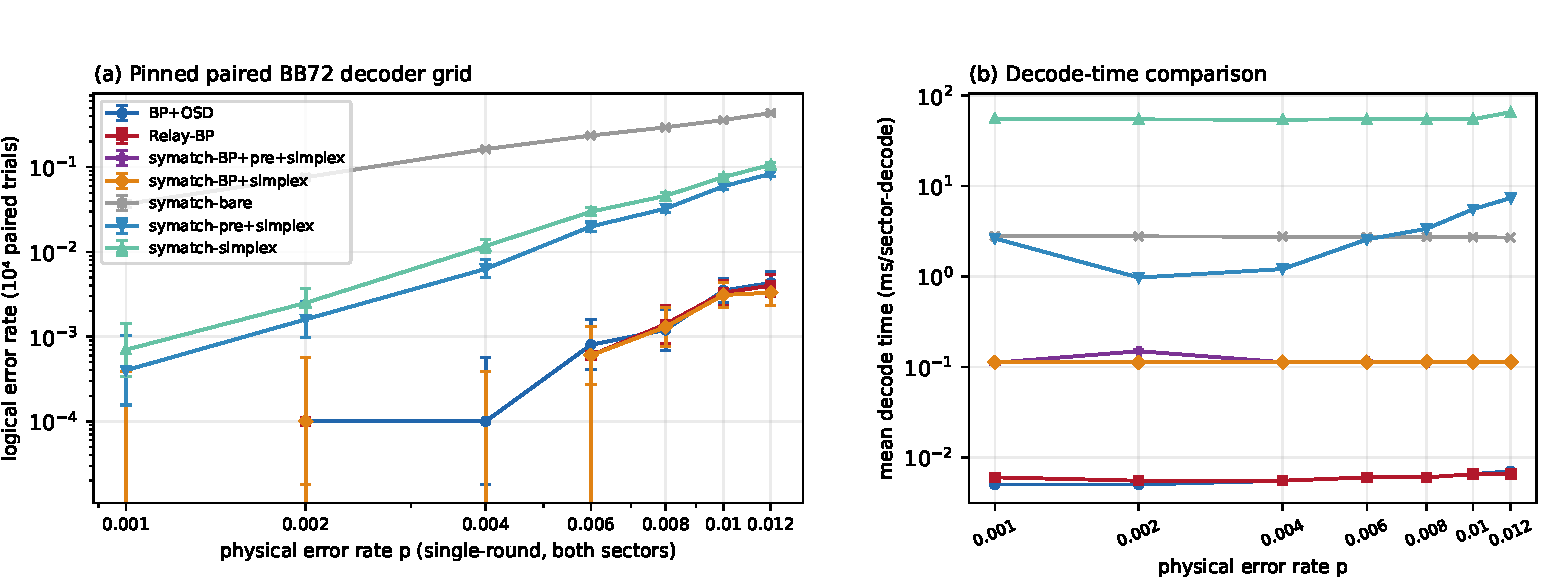
\includegraphics[width=\columnwidth]{figures/cmp_f1_grid_final.pdf}
\caption{(a) Pinned paired BB72 decoder grid with Wilson 95\% confidence intervals; (b) per-sector decode time from a single-process probe. Under these implementations, the measured matching-core decoders take $10^2$--$10^4$ times as long per decode as the BP-family decoders. Bare matching has substantially higher LFR, while the observed differences for BP-augmented variants lie within the reported $\pm0.5$ percentage-point margin; because the margin was selected after the initial grid, this is descriptive rather than confirmatory evidence of equivalence.}
\label{fig:grid}
\end{figure}

%%-----------------------------------------------------------
\subsection{Repeated-cycle BP+OSD benchmark}
\label{sec:rc}
%%-----------------------------------------------------------

We now test BP+OSD when data and measurement faults accumulate over repeated syndrome rounds, reporting a fixed-sample grid, a separately analyzed adaptive extension, and a finite-size upward extension that resolves the crossover directly. The aim throughout is to characterize the tested implementations and operating range under the pinned protocol.

\noindent\textbf{Repeated-cycle protocol.} We use QEC Emulator's \texttt{run\_repeated\_cycle}~\cite{AlDaajeh2026emulator}. Each trial contains $d$ syndrome rounds, with $d=6$, 12, and 18 for BB72, BB144, and BB288, respectively. Rounds $1$ through $d-1$ apply Bernoulli faults at rate $p$ to data and measurement bits; the final round is noiseless. Decoding uses the space-time check matrix in Eq.~(\ref{eq:spacetime}). The fixed grid uses 2{,}000 trials per point for BB72 and BB144 and 500 for BB288.

\noindent\textbf{Fixed-grid results.} Table~\ref{tab:rc} reports the prespecified fixed-sample grid; the adaptive extension used to resolve lower failure rates follows, and the upward extension that localizes the crossover is the subject of Section~\ref{ssec:fss}.

\begin{table}[htbp]\centering\small
\caption{Repeated-cycle BP+OSD, $d$~rounds per trial, Wilson 95\% CIs (nonzero rows); zero-failure rows report the exact one-sided 95\% Clopper--Pearson UB $2.996/N$ (Remark~\ref{rem:zerofail}): $<0.00150$ ($n=2{,}000$); $<0.00599$ ($n=500$). Grid with exactly aligned spacetime priors (\texttt{model\_rev=aligned-priors}; final-round fault variables removed, all surviving priors $=p$). Files: \texttt{repeated\_cycle\_bposd.csv}, \texttt{repeated\_cycle\_bb288\_bposd.csv}, \texttt{repeated\_cycle\_all\_codes.csv}.}\label{tab:rc}
\begin{tabular}{@{}lrrrll@{}}
\toprule
Code (rounds, trials) & $p$ & Failures & LFR & Wilson 95\% CI \\\midrule
BB72 ($d=6$,$n=2000$)   & 0.001 &  0 & $<$0.00150 & exact CP UB \\
BB72 ($d=6$,$n=2000$)   & 0.002 &  0 & $<$0.00150 & exact CP UB \\
BB72 ($d=6$, $n=2000$)   & 0.004 &  1 & 0.00050 & [0.00009,\;0.00283] \\
BB72 ($d=6$, $n=2000$)   & 0.006 &  3 & 0.00150 & [0.00051,\;0.00440] \\
BB72 ($d=6$, $n=2000$)   & 0.008 & 10 & 0.00500 & [0.00272,\;0.00918] \\
BB72 ($d=6$, $n=2000$)   & 0.010 & 24 & 0.01200 & [0.00808,\;0.01779] \\
BB72 ($d=6$, $n=2000$)   & 0.012 & 37 & 0.01850 & [0.01345,\;0.02540] \\\midrule
BB144 ($d=12$,$n=2000$) & 0.001-0.012 & 0 each & $<$0.00150 & exact CP UB (all 7 pts) \\\midrule
BB288 ($d=18$,$n=500$)  & 0.001-0.012 & 0 each & $<$0.00599 & exact CP UB (all 7 pts) \\
\bottomrule
\end{tabular}
\end{table}

At $p=0.008$, the fixed grid records 10 failures in 2{,}000 BB72 trials, none in 2{,}000 BB144 trials, and none in 500 BB288 trials. The corresponding 95\% upper bounds for the zero-count rows are $0.15\%$ and $0.60\%$, respectively; these bounds reflect the different sample sizes and do not establish zero risk. Across the full grid, BB144 and BB288 have no observed failures, while BB72's LFR increases with $p$. All fixed-grid trial counts were set in advance.

\noindent\textbf{Adaptive extension.} To obtain more informative estimates beyond the fixed-sample grid, a separate campaign adaptively accumulated batches until reaching its stopping criterion. Because optional stopping changes interval coverage, these results use time-uniform confidence sequences rather than fixed-sample Wilson intervals.

\begin{table}[htbp]\centering\small
\caption{Repeated-cycle adaptive extension (E3, prior-aligned grid): $d$~rounds per trial, 2{,}000-trial batches, stopping at $\ge50$ failures or 20{,}000 trials; batch seeds \texttt{stable\_seed(`E3',\,code,\,$p$,\,rounds,\,batch)} (the $p=0.010$ rows use tag \texttt{E3p010}). All rows: 95\% Robbins uniform-mixture confidence sequences~\cite{howard2021confidence}, time-uniform and valid under the pinned stopping rule (fixed-sample formulas would not be valid: nominal-95\% Wilson coverage under this rule is $\approx\!93.9\%$ at $p=0.021$, \texttt{stats\_intervals.py -self-check}); zero rows report the CS upper endpoint $6.45\times10^{-4}$ ($n=20{,}000$). Files: \texttt{repeated\_cycle\_adaptive\_*.csv} (raw counts), \texttt{rc\_adaptive\_cs.csv} (intervals).}\label{tab:rc_adaptive}
\begin{tabular}{@{}lrrrll@{}}
\toprule
Code (rounds) & $p$ & Failures & Trials & LFR & 95\% confidence sequence \\\midrule
BB72 ($d=6$)   & 0.004 & 16 & 20{,}000 & $8.0\times10^{-4}$ & $[0.19,2.10]\times10^{-3}$ \\
BB72 ($d=6$)   & 0.006 & 60 & 20{,}000 & $3.0\times10^{-3}$ & $[1.59,5.07]\times10^{-3}$ \\
BB72 ($d=6$)   & 0.008 & 62 & 10{,}000 & $6.2\times10^{-3}$ & $[3.41,10.2]\times10^{-3}$ \\
BB72 ($d=6$)   & 0.010 & 64 & 4{,}000  & $1.60\times10^{-2}$ & $[9.20,25.5]\times10^{-3}$ \\
BB72 ($d=6$)   & 0.012 & 84 & 4{,}000  & $2.10\times10^{-2}$ & $[13.1,31.5]\times10^{-3}$ \\\midrule
BB144 ($d=12$) & 0.004 & 0 & 20{,}000 & $<$$6.45\times10^{-4}$ & CS upper endpoint \\
BB144 ($d=12$) & 0.006 & 1 & 20{,}000 & $5.0\times10^{-5}$ & $[{\sim}0,\;7.82]\times10^{-4}$ \\
BB144 ($d=12$) & 0.008 & 0 & 20{,}000 & $<$$6.45\times10^{-4}$ & CS upper endpoint \\
BB144 ($d=12$) & 0.010 & 2 & 20{,}000 & $1.0\times10^{-4}$ & $[{\sim}0,\;8.99]\times10^{-4}$ \\
BB144 ($d=12$) & 0.012 & 4 & 20{,}000 & $2.0\times10^{-4}$ & $[4.5\times10^{-6},\,1.10\times10^{-3}]$ \\\midrule
BB288 ($d=18$) & 0.004 & 0 & 20{,}000 & $<$$6.45\times10^{-4}$ & CS upper endpoint \\
BB288 ($d=18$) & 0.006 & 0 & 20{,}000 & $<$$6.45\times10^{-4}$ & CS upper endpoint \\
BB288 ($d=18$) & 0.008 & 0 & 20{,}000 & $<$$6.45\times10^{-4}$ & CS upper endpoint \\
BB288 ($d=18$) & 0.010 & 0 & 20{,}000 & $<$$6.45\times10^{-4}$ & CS upper endpoint \\
BB288 ($d=18$) & 0.012 & 0 & 20{,}000 & $<$$6.45\times10^{-4}$ & CS upper endpoint \\
\bottomrule
\end{tabular}
\end{table}

\noindent\textbf{Finite-size evidence and scope.} Taken together with the single-round comparisons in Section~\ref{sec:benchmark}, the fixed and adaptive grids provide finite-size evidence for suppression of logical failures with increasing code size under the tested phenomenological protocols. For example, at $p=0.008$ the single-round grid records 14/10{,}000 failures for BB72 and zero observed failures for BB144 and BB288; the repeated-cycle grid records 10/2{,}000 for BB72 and zero for the larger codes. Zero-count results are upper bounds whose strength depends on the trial count, so they do not establish a strict population-risk ordering at every rate. Section~\ref{ssec:fss} converts this ordering evidence into a measured crossing phenomenon by extending the identical protocol to higher error rates.

\noindent\textbf{Distance-ladder suppression factor \texorpdfstring{$\Lambda$}{Lambda}.} For the adaptive distance ladder $d=6,12,18$, we define $\Lambda$ through the per-block failure ratios
\[
\frac{\mathrm{LFR}_{d}}{\mathrm{LFR}_{d+6}}=\Lambda^3,
\qquad
\frac{\mathrm{LFR}_{6}}{\mathrm{LFR}_{18}}=\Lambda^6.
\]
Thus, $\Lambda$ is the geometric-mean suppression per two-round increment across a six-round gap, not a per-cycle suppression factor. The surface-code value $\Lambda=2.14\pm0.02$~\cite{Acharya2024lambda} comes from circuit-level hardware data under a different protocol; we cite it only as context and make no quantitative performance comparison.

All ladder arms use adaptive stopping, so inference is based on time-uniform confidence sequences, with four-endpoint Bonferroni correction for two-sided ratios and two-endpoint correction for one-sided bounds~\cite{howard2021confidence}; implementation details are in \texttt{stats\_intervals.py}. At $p=0.004$, the BB72-to-BB144 ratio is unresolved because its confidence-sequence lower bound is below one. For the remaining tested rates, the BB72-to-BB144 observed suppression and lower bounds are: $60\times$ observed and $>1.77\times$ ($\Lambda=3.91$ observed, $\Lambda>1.21$) at $p=0.006$; lower bound $>4.9\times$ ($\Lambda>1.70$) at $p=0.008$; $160\times$ observed and $>9.0\times$ ($\Lambda=5.43$ observed, $\Lambda>2.08$) at $p=0.010$; and $105\times$ observed and $>10.6\times$ ($\Lambda=4.72$ observed, $\Lambda>2.19$) at $p=0.012$. Upper bounds are uninformative when the higher-distance arm has only $O(1)$ failures, so observed ratios and lower bounds are reported separately.

On the initial ladder, which terminates at $p=0.012$, the BB144-to-BB288 rung is not statistically resolved at 20{,}000 trials per point: BB288 has zero failures at every tested rate, while BB144 has only 1, 2, and 4 failures at $p=0.006$, 0.010, and 0.012, respectively; the resulting one-sided ratio bounds are vacuous, and no point estimate is reported. For the two-step BB72-to-BB288 comparison, the lower bounds are $>18.9\times$ ($\Lambda>1.63$) at $p=0.012$, $>13.2\times$ ($\Lambda>1.54$) at $p=0.010$, and $>4.9\times$ ($\Lambda>1.30$) at $p=0.008$. The upward extension of Section~\ref{ssec:fss} resolves the second rung directly at higher error rates, where both arms fail often enough for informative ratios.

%%-----------------------------------------------------------
\subsection{Finite-size extension: measured curve crossings}
\label{ssec:fss}
%%-----------------------------------------------------------

The adaptive ladder of Table~\ref{tab:rc_adaptive} terminates at $p=0.012$ with strict size ordering and no crossing, which bounds but does not localize the crossover. We therefore extended the same experiment upward in physical error rate, holding every element of the protocol fixed---the aligned-priors spacetime matrices, the perfect final round, min-sum BP at scaling $0.625$ with OSD-CS order~7, $d$ rounds per trial, 2{,}000-trial batches, and the $\ge50$-failure adaptive stop---and varying only the grid, to $p\in\{0.016,0.020,0.024,0.028,0.032\}$ for all three codes and $p\in\{0.036,0.040,0.045,0.050\}$ for BB72 and BB144, under an independent seed stream (\texttt{stable\_seed(`E3fss',\,\ldots)}). The BB288 cells use a pinned 6{,}000-trial budget (Section~\ref{sec:limitations}). Table~\ref{tab:fss} reports the extended ladder.

\begin{table}[htbp]\centering\small
\caption{Finite-size extension of the repeated-cycle ladder (identical protocol, independent seed stream): $d$~rounds per trial, adaptive batches of 2{,}000, stopping at $\ge50$ failures or the pinned budget; Wilson 95\% intervals (fixed-sample; every extended cell completed its stopping rule without early-termination ambiguity---the $\ge50$-failure cells stopped at the batch boundary shown). The suppression ratio $R=\mathrm{LFR}_{d}/\mathrm{LFR}_{d+6}$ and $\Lambda=R^{1/3}$ follow the block-$\Lambda$ convention of Section~\ref{sec:rc} and are evaluated on the first rung ($d{=}6$ vs $d{=}12$). BB288 cells use a pinned 6{,}000-trial budget; failure-free cells ($\dagger$) report the exact Clopper--Pearson 95\% upper bound, and cells at $p\ge0.032$ reached the $\ge50$-failure stop after one 2{,}000-trial batch. Files: \texttt{repeated\_cycle\_fss\_*.csv}, \texttt{repeated\_cycle\_fss\_hip\_bb288.csv}.}
\label{tab:fss}
\setlength{\tabcolsep}{2.5pt}
\begin{tabular}{@{}rlllll@{}}
\toprule
$p$ & BB72 ($d{=}6$) LFR [Wilson] & BB144 ($d{=}12$) LFR [Wilson] & BB288 ($d{=}18$) LFR [Wilson] & $R$ & $\Lambda=R^{1/3}$ \\\midrule
0.016 & 0.0620 [0.0522,\,0.0734] & 0.0015 [0.0011,\,0.0021] & $0$ [$0$,\,$5.0{\times}10^{-4}$]$^{\dagger}$ & 41.3$\times$ & 3.46 \\
0.020 & 0.0975 [0.0853,\,0.1113] & 0.0060 [0.0047,\,0.0077] & $0$ [$0$,\,$5.0{\times}10^{-4}$]$^{\dagger}$ & 16.3$\times$ & 2.53 \\
0.024 & 0.1615 [0.1460,\,0.1783] & 0.0200 [0.0161,\,0.0248] & 0.0005 [0.0002,\,0.0015] & \phantom{0}8.1$\times$ & 2.01 \\
0.028 & 0.2800 [0.2608,\,0.3001] & 0.0740 [0.0633,\,0.0863] & 0.0087 [0.0066,\,0.0113] & \phantom{0}3.8$\times$ & 1.56 \\
0.032 & 0.4170 [0.3956,\,0.4387] & 0.1895 [0.1729,\,0.2073] & 0.0925 [0.0806,\,0.1060] & \phantom{0}2.2$\times$ & 1.30 \\
0.036 & 0.5415 [0.5196,\,0.5632] & 0.4220 [0.4005,\,0.4438] & 0.4500 [0.4283,\,0.4719] & \phantom{0}1.28$\times$ & 1.09 \\
0.040 & 0.6540 [0.6329,\,0.6745] & 0.7140 [0.6938,\,0.7334] & 0.8895 [0.8750,\,0.9025] & \phantom{0}0.92$\times$ & 0.97 \\
0.045 & 0.8215 [0.8041,\,0.8377] & 0.9355 [0.9239,\,0.9455] & 0.9985 [0.9956,\,0.9995] & \phantom{0}0.88$\times$ & 0.96 \\
0.050 & 0.9110 [0.8977,\,0.9227] & 0.9940 [0.9895,\,0.9966] & 1.0000 [0.9981,\,1.0000] & \phantom{0}0.92$\times$ & 0.97 \\
\bottomrule
\end{tabular}
\end{table}

Three features of Table~\ref{tab:fss} constitute the finite-size scaling evidence. First, the size ordering is strict and statistically separated throughout the sub-crossover window: at every $p\le0.032$ the Wilson intervals of all three adjacent rungs are pairwise disjoint, and BB288 is failure-free at $p\le0.020$ (0/6{,}000 at both $p=0.016$ and $p=0.020$, exact Clopper--Pearson upper bound $5.0\times10^{-4}$) and strongly suppressed through the rest of the sub-crossover window---$3/6{,}000$ at $p=0.024$, $52/6{,}000$ at $p=0.028$, $0.0925$ at $p=0.032$. Second, the suppression factor collapses monotonically toward unity as the crossover is approached, $\Lambda=3.46\to1.09$ over $p=0.016\to0.036$---the signature of a genuine critical region rather than a uniform performance gap; the second rung shows the same collapse where resolvable ($R_{12,18}=40\times\to2.0\times$, i.e.\ $\Lambda_{12,18}=3.42\to1.27$ over $p=0.024\to0.032$). Third, the $d{=}6$ and $d{=}12$ curves cross inside the window: the ordering is intact at $p=0.036$ (intervals $[0.520,0.563]$ vs $[0.401,0.444]$) and inverted at $p=0.040$ ($[0.633,0.675]$ vs $[0.694,0.733]$), both with disjoint intervals, bracketing the crossover at $p_{\times}\in(0.036,0.040)$; linear interpolation on the LFR difference places it at $p_{\times}\approx0.039$.

We therefore read the bracket as localizing, not merely lower-bounding, the threshold of this decoder--model combination. The second-rung crossing is measured as well: the $d{=}12/18$ ordering is intact at $p=0.032$ with disjoint intervals ($0.0925$ $[0.081,0.106]$ versus $0.1895$ $[0.173,0.207]$) and inverted at $p=0.036$ ($0.450$ $[0.428,0.472]$ versus $0.422$ $[0.401,0.444]$; point estimates inverted, intervals overlapping), bracketing $p_{\times}(12,18)\in(0.032,0.036)$ with interpolation $\approx0.035$. The two successive crossings, $p_{\times}(6,12)\approx0.039$ and $p_{\times}(12,18)\approx0.035$, are mutually consistent---separated by less than one grid step---and jointly localize the threshold region to $(0.032,0.040)$; we report a measured crossing region and do not extrapolate a drift direction from two rungs. The estimate is specific to the noise model and decoder (phenomenological spacetime noise at rate $p$ per round, min-sum BP+OSD at the pinned operating point) and makes no circuit-level claim. The bracket is consistent with independent anchors: the code-capacity threshold of the weight-six $k{=}12$ BB family under BP-OSD is $8.38(6)\%$~\cite{English2026duality}, and a spacetime model with noisy measurements is expected to cross lower. Within that scope, the statement is no longer qualitative ordering: it is a measured curve crossing on two successive rungs---the first fully interval-separated, the second interval-separated at its lower endpoint---with suppression factors collapsing to unity on both, obtained under one pinned protocol across three code sizes.

%%-----------------------------------------------------------
\subsection{Circuit-level decoder evaluation}
\label{sec:circuit}

The single-round and paired-grid results above use code-capacity noise. We next examine two distinct circuit-level sources: a re-analysis of a published detector error model and a synthetic BB72 circuit. Together they test how the observed decoder behavior carries over to circuit-derived data, while keeping the two evidence sources clearly separate.

\noindent\textbf{Arm A: released Kunlun detector-model re-analysis.} This arm re-analyses the released detector error model, not raw hardware shots. The Kunlun collaboration published the complete detector check matrices and per-mechanism channel probabilities for its $[[18,4,4]]$ BB hardware experiment~\cite{Wang2026kunlun} (Zenodo, CC-BY-4.0); our results are Monte Carlo samples from that published model, decoded independently. No new hardware data are involved, and we make no claim about the Kunlun device beyond the released model. We sampled 10{,}000 shots per point at 1, 3, and 6 QEC rounds in both sectors, using five decoders: BP+OSD (the authors' configuration, $10^4$ iterations, CS-7), BP-only, static-prior MWPM on the chain-graphified DEM, belief-matching~\cite{Higgott2023belief} (which reweights the matching graph per shot using BP posteriors), and Relay-BP~\cite{Muller2025relay}. Results are in \texttt{kunlun\_cmp.csv} and Figure~\ref{fig:kunlun}.

\begin{table}[!htbp]\centering\small
\caption{Five decoders on the published Kunlun $[[18,4,4]]$ DEM, 10{,}000 shots per point. Bold: best (or statistically tied-best) per row. Ordering Relay-BP $\leq$ BP+OSD $<$ BP-only $\ll$ BeliefMatch $<$ MWPM holds in all six configurations.}
\label{tab:kunlun}
\begin{tabular}{@{}llrrrrr@{}}
\toprule
Rounds & Sector & Relay-BP & BP-OSD & BP-only & BeliefMatch & MWPM-prior \\\midrule
1 & X & \textbf{0.2082} & 0.2103 & 0.2324 & 0.4231 & 0.4270 \\
1 & Z & \textbf{0.2223} & 0.2248 & 0.2502 & 0.5299 & 0.5365 \\
3 & X & \textbf{0.5489} & \textbf{0.5489} & 0.5897 & 0.7507 & 0.7653 \\
3 & Z & \textbf{0.5123} & 0.5190 & 0.5626 & 0.7836 & 0.8155 \\
6 & X & \textbf{0.7887} & 0.7952 & 0.8208 & 0.8921 & 0.9026 \\
6 & Z & \textbf{0.7670} & 0.7728 & 0.8111 & 0.9109 & 0.9237 \\
\bottomrule
\end{tabular}
\end{table}

Three conclusions follow. \textbf{(i)} The graphification penalty measured in Section~\ref{sec:benchmark} is not an artifact of our synthetic DEM: on the authors' hardware DEM, matching-family decoders are $2.0$-$2.4\times$ worse than BP+OSD at round 1, the penalty decaying to $1.1$-$1.2\times$ by round 6 as the LER saturates; early rounds carry the information. \textbf{(ii)} Per-shot belief reweighting recovers only 0.4-3.2 percentage points over the static-prior matching baseline, quantitatively mirroring the modest decoder-side gains of the defect-aware arm in~\cite{Bartlett2026defect} on independent hardware. \textbf{(iii)} Relay-BP matches or beats the $10^4$-iteration BP+OSD reference at $\sim\!35\times$ lower wall time per point (8~s vs 288~s average, same machine, single process, identical inputs), consistent with its real-time design goal~\cite{Muller2025relay,Johnson2026relayfpga}.

\begin{figure}[H]\centering
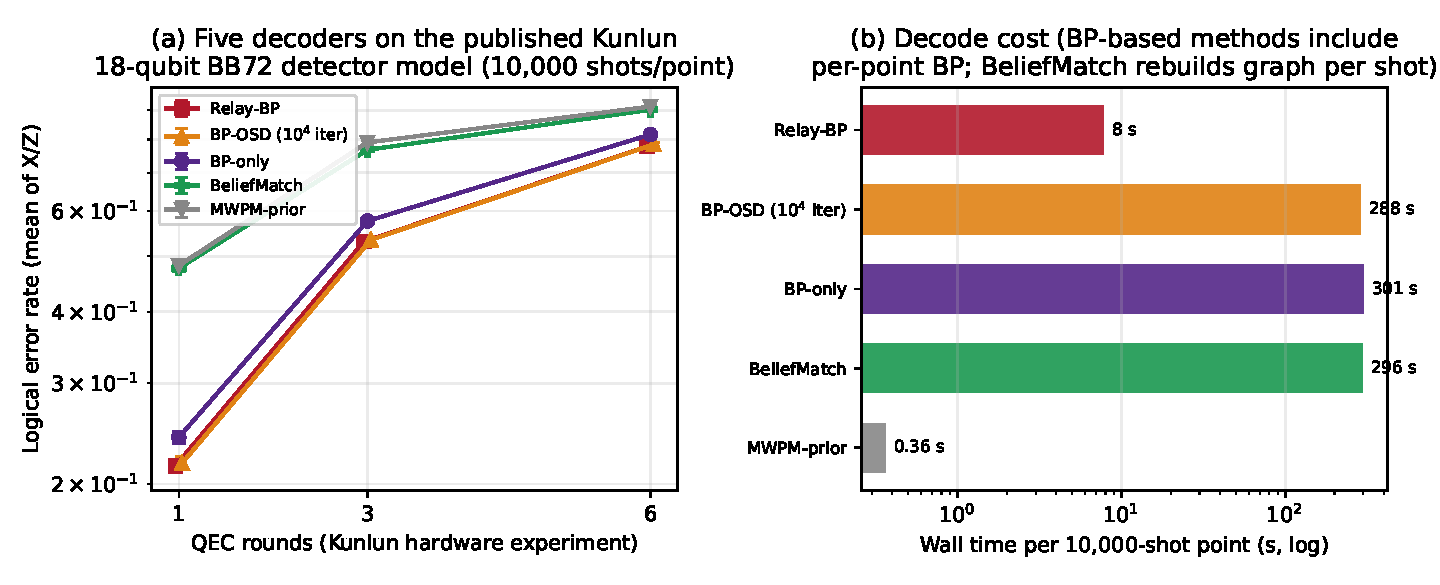
\includegraphics[width=\columnwidth]{figures/cmp_f2_kunlun.pdf}
\caption{(a) Five decoders on the Kunlun hardware DEM, mean of X/Z sectors, Wilson 95\% CIs; (b) wall time per 10{,}000-shot point.}
\label{fig:kunlun}
\end{figure}

\noindent\textbf{Arm B: synthetic BB72 circuit-level point.} This arm tests the code-capacity graphification penalty from Section~\ref{sec:benchmark} in a synthetic BB72 $Z$-memory circuit with four extraction rounds, DEPOLARIZE1/2 gate noise, measurement flips at rate $p$, data-idle noise during measurement windows, and a serial-by-check schedule. Reset and preparation are ideal; their errors are not modeled. The circuit is compiled with Stim~\cite{Gidney2021} and sampled for 20{,}000 shots per rate; BP+OSD, Relay-BP, belief-matching, and two matching baselines decode the resulting syndromes. Four protocol-invariance test groups validate the extraction circuit: gadget parity (a reversed primitive returns input-independent zero), codespace silence, injection-column alignment with $H_Z$/$H_X$, and a detector/observable map audit. All tests pass deterministically (\texttt{wsc\_verify.py}, \texttt{wsc\_verify\_report.json}). The campaign is checkpointed and resume-safe, with per-point DEM digests; here we report the completed and verified $p=0.001$ operating point (\texttt{wsc\_circuit.csv}; Figure~\ref{fig:wsc}).

\begin{table}[htbp]\centering\small
\caption{Synthetic BB72 circuit-level $Z$-memory, 4 rounds, 20{,}000 shots, validated extraction (four invariance test groups; \texttt{wsc\_verify.py}). Failures (LER); zero-failure rows report the exact one-sided 95\% Clopper--Pearson UB (Remark~\ref{rem:zerofail}). MWPM-stim failures are entirely coverage failures (see text).}
\label{tab:wsc}
\begin{tabular}{@{}lrrrrr@{}}
\toprule
$p$ & BP+OSD & Relay-BP & BeliefMatch & MWPM-chain & MWPM-stim \\
\midrule
0.001 & 51 (0.0026) & 0 ($<$$1.50\!\times\!10^{-4}$) & 12826 (0.6413) & 12848 (0.6424) & 13824 (0.6912) \\
\bottomrule
\end{tabular}
\end{table}

Three findings. \textbf{(i) The naive-reduction penalty is catastrophic at circuit level}: at $p=0.001$ the chain-graphified matching decoder fails 64.2\% of shots versus 0.255\% for BP+OSD; a 252$\times$ penalty. \textbf{(ii) Relay-BP's advantage is a circuit-level phenomenon}: under code-capacity noise (Section~\ref{sec:comparator}) Relay-BP and BP+OSD are statistically tied, but on this circuit DEM Relay-BP fails zero of 20{,}000 shots (exact CP UB $1.50\times10^{-4}$) while BP+OSD sits at $2.55\times10^{-3}$ (Wilson CI $[1.94,3.35]\times10^{-3}$, excluding the Relay-BP UB) on identical shots; quantitatively consistent with the circuit-level superiority reported in~\cite{Muller2025relay} and, on this tested operating point, associating that superiority with the noise model rather than the code; we do not extrapolate a general decoder ordering from a single circuit operating point. \textbf{(iii) The standard matching toolchain cannot even be instantiated natively}: Stim's hyperedge decomposition fails on this DEM outright (weight-6 checks induce correlated mechanisms that do not decompose); with \texttt{ignore\_decomposition\_failures} the dropped mechanisms leave 69.1\% of shots without any perfect matching at $p=0.001$ (every such shot is a counted failure, and all 13{,}824 MWPM-stim failures are of this form). Within the tested reductions and this pinned circuit configuration, weight-6-check qLDPC circuits therefore sit outside the representational reach of the pairwise-matching stack: both tested routes to a pairwise model (Stim's native hyperedge decomposition and the independent-merge chain graphification) either fail outright or discard the correlated mechanisms, and BP-family decoders are the only operable option among those tested. We do not claim that no bespoke pairwise reduction exists; a general inexpressiveness statement would require a formal argument beyond the tested constructions.

\begin{figure}[H]\centering
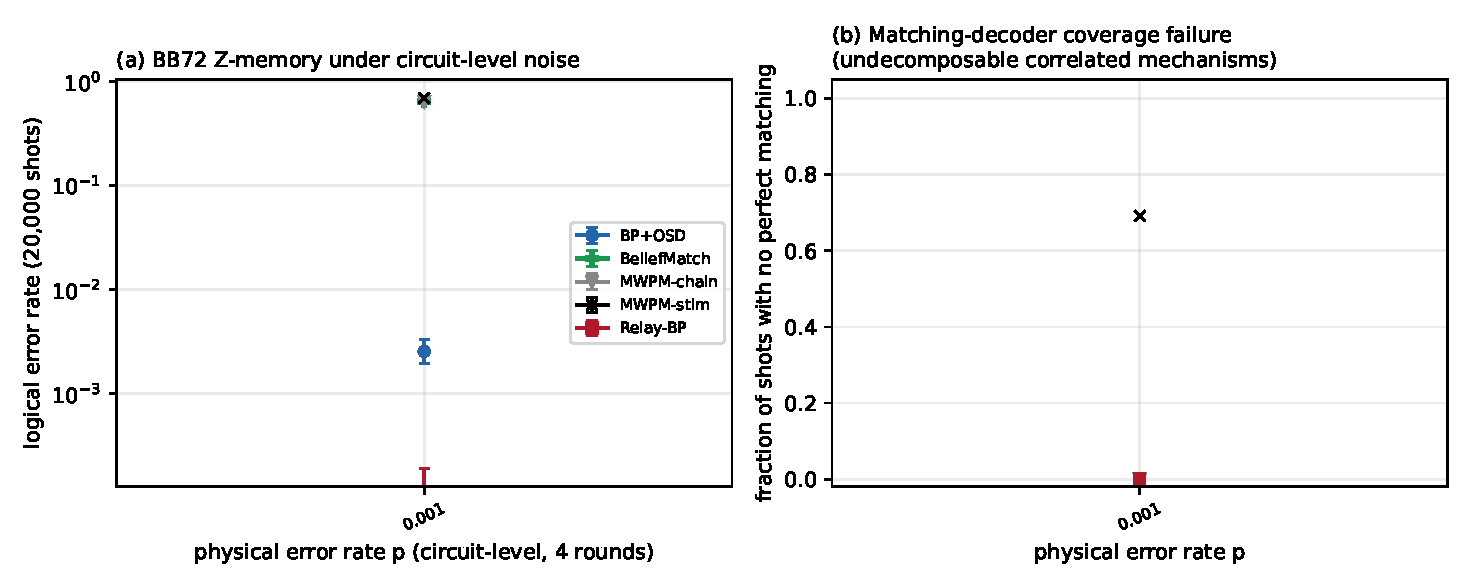
\includegraphics[width=\columnwidth]{figures/cmp_f3_wsc.pdf}
\caption{(a) BB72 circuit-level $Z$-memory LER, Wilson 95\% CIs; (b) fraction of shots for which no perfect matching exists.}
\label{fig:wsc}
\end{figure}

\subsection{Hardware-informed noise simulations and ablations}
\label{sec:hardware}
%%-----------------------------------------------------------

This section examines how hardware-inspired noise components affect simulated single-cycle BB72 logical failure rates. It complements the decoder and circuit-level comparisons by testing the sensitivity of those rates to selected model assumptions; on its own it is not a real-device experiment, and its causal conversion is the subject of Section~\ref{sec:causal}. We distinguish three analyses: component ablations in the effective-mask \texttt{HardwareModel}, reset sensitivity in the schedule-level \texttt{CircuitLevelModel}, and a rate sweep comparing phenomenological, CZ, and MS noise models. Because these are separate Monte Carlo studies under different model assumptions, conclusions are restricted to the corresponding configurations and operating points.

\noindent\textbf{Component ablations.} The effective-mask ablation varies four modeled contributions one at a time at $p_{\mathrm{base}}=5\times10^{-4}$, with 3{,}000 trials per condition and a radius-2 lookup decoder. The factors are: (1)~\emph{SWAP routing overhead}, arising from nonlocal check routing in the planar CZ architecture (approximately 96 SWAPs among 432 two-qubit gates per cycle); (2)~\emph{gate decoherence}, with thermal relaxation and dephasing during gates ($p_1\approx1.33\times10^{-3}$ per CZ gate and negligible contribution for MS); (3)~\emph{idle noise}, set to $p_{\mathrm{idle}}=0.05p_{\mathrm{base}}$; and (4)~\emph{measurement noise}, with ancilla readout error $p_{\mathrm{meas}}=p_{\mathrm{base}}$.

Table~\ref{tab:ablation} shows the resulting model-specific sensitivities. The CZ full-model condition yields 30 failures in 3{,}000 trials (LFR $=0.0100$), compared with 15 when SWAP overhead is removed (LFR $=0.0050$) and 7 when measurement noise is removed (LFR $=0.0023$). These observed changes are $0.0050$ and approximately $0.0077$, respectively. Removing idle noise leaves the count unchanged at 30, so this experiment detects no idle-noise effect at the tested setting---a model-level observation that the causal campaign of Section~\ref{sec:causal} later confirms on device (Arm~D), rather than a proof that idle noise is generally negligible. The gate-decoherence-only arm has zero failures, corresponding to an exact one-sided 95\% Clopper--Pearson upper bound below $0.000999$, rather than a precise estimate of that component's contribution. For MS, matching the CZ gate-error parameters increases the observed LFR from $0.0023$ to $0.0063$. Together, these contrasts indicate sensitivity to routing, readout, and gate-error parameters within this model, but the one-factor-at-a-time design does not isolate interactions or support attribution of a physical-device gap to any single mechanism.

\begin{table}[htbp]\centering\small
\caption{Effective-mask hardware-model ablations for BB72 at $p_{\mathrm{base}}=5\times10^{-4}$, with 3{,}000 trials per condition and a radius-2 lookup decoder. Zero failures are reported with the exact one-sided 95\% Clopper--Pearson upper bound. Results characterize this simulation model only. File: \texttt{hardware\_ablations.csv}.}
\label{tab:ablation}
\begin{tabular}{@{}lrrr@{}}
\toprule
Condition & Failures & LFR & Wilson 95\% CI \\
\midrule
Phenomenological baseline   &  3 & 0.0010 & [0.00034,\;0.00294] \\
CZ: full model              & 30 & 0.0100 & [0.00701,\;0.01424] \\
CZ: no SWAP overhead        & 15 & 0.0050 & [0.00303,\;0.00823] \\
CZ: no idle noise           & 30 & 0.0100 & [0.00701,\;0.01424] \\
CZ: no measurement noise    &  7 & 0.0023 & [0.00113,\;0.00481] \\
CZ: gate decoherence only   &  0 & $<$0.000999 & exact CP UB (Rem.~\ref{rem:zerofail}) \\
MS: full model              &  7 & 0.0023 & [0.00113,\;0.00481] \\
MS: CZ-matched gate error   & 19 & 0.0063 & [0.00406,\;0.00987] \\
\bottomrule
\end{tabular}
\end{table}

A separate reset-sensitivity study tests preparation noise in the schedule-level \texttt{CircuitLevelModel}, which propagates preparation faults through the circuit. It uses BB72, $p=5\times10^{-4}$, 3{,}000 trials per condition, a radius-2 lookup decoder, and pinned seeds (Table~\ref{tab:reset}). The observed LFR rises from $0.0637$ without reset noise to $0.0827$ at the nominal setting and $0.1077$ when reset noise is doubled; the corresponding Wilson intervals are separated for adjacent settings. At matched nominal syndrome-noise rates, reset-only and readout-only conditions yield LFRs of $0.0900$ and $0.0670$, with non-overlapping intervals. This supports a distinct logical effect from preparation faults under this schedule, but does not by itself identify all reset, readout, and idle interactions. The no-readout condition (288/3{,}000) is slightly above the full-model condition (248/3{,}000), but their intervals overlap and the trials are unpaired, so this difference is not interpreted as evidence of an increase. Absolute rates from this circuit-level study are not directly comparable with the effective-mask ablation above because the fault models and propagation mechanisms differ.

\begin{table}[htbp]\centering\small
\caption{Reset-sensitivity Monte Carlo for BB72 in the schedule-level circuit model at $p=5\times10^{-4}$, with 3{,}000 trials per condition and a radius-2 lookup decoder. File: \texttt{reset\_sensitivity.csv}.}
\label{tab:reset}
\begin{tabular}{@{}lrrr@{}}
\toprule
Condition & Failures & LFR & Wilson 95\% CI \\
\midrule
circuit: full model        & 248 & 0.0827 & [0.07334,\;0.09306] \\
circuit: no reset noise    & 191 & 0.0637 & [0.05548,\;0.07297] \\
circuit: reset $\times2$   & 323 & 0.1077 & [0.09707,\;0.11926] \\
circuit: no readout        & 288 & 0.0960 & [0.08597,\;0.10706] \\
circuit: reset-only syn    & 270 & 0.0900 & [0.08028,\;0.10077] \\
circuit: readout-only syn  & 201 & 0.0670 & [0.05860,\;0.07651] \\
\bottomrule
\end{tabular}
\end{table}

\noindent\textbf{Single-cycle operating-point comparison.} To place these sensitivities in context, Table~\ref{tab:hw} compares single-cycle BB72 LFR across phenomenological, CZ, and MS noise models over five physical-noise settings. Each point uses 5{,}000 trials and the radius-2 lookup decoder. The CZ model has a higher observed LFR than the MS model at every tested rate, and their reported 95\% intervals do not overlap at any of the five rates. This is evidence about the specified simulated models, not a claim that one gate family is intrinsically less error-prone on hardware.

\begin{table}[htbp]\centering\small
\caption{Single-cycle BB72 LFR comparison across phenomenological, CZ, and MS noise models; 5{,}000 trials per rate and a radius-2 lookup decoder. Each cell gives failures and a 95\% confidence interval for LFR in units of $10^{-3}$; nonzero cells use Wilson intervals and zero-failure cells the exact two-sided Clopper--Pearson upper bound. The CZ and MS intervals do not overlap at any tested rate. File: \texttt{hardware\_three\_condition\_comparison.csv}.}
\label{tab:hw}
\begin{tabular}{@{}lrrr@{}}
\toprule
$p$ & Phenomenological & CZ & MS \\\midrule
$5\!\times\!10^{-4}$ & $0\;(<0.77)$ & $10\;[1.09,3.68]$ & $0\;(<0.77)$ \\
$1\!\times\!10^{-3}$ & $2\;[0.11,1.46]$ & $15\;[1.82,4.94]$ & $0\;(<0.77)$ \\
$2\!\times\!10^{-3}$ & $1\;[0.04,1.13]$ & $46\;[6.90,12.25]$ & $8\;[0.81,3.15]$ \\
$3\!\times\!10^{-3}$ & $14\;[1.67,4.69]$ & $77\;[12.34,19.20]$ & $6\;[0.55,2.62]$ \\
$5\!\times\!10^{-3}$ & $70\;[11.10,17.65]$ & $171\;[29.51,39.61]$ & $52\;[7.94,13.61]$ \\
\bottomrule
\end{tabular}
\end{table}

The phenomenological-model counts are non-monotone between $p=10^{-3}$ and $2\times10^{-3}$ (2 and 1 failures, respectively). The intervals overlap, and each point uses a separate fixed-size Monte Carlo sample; accordingly, we report the raw estimates without smoothing or imposing monotonicity.

%%-----------------------------------------------------------
\section{Causal hardware ablation on ibm\_marrakesh}
\label{sec:causal}
%%-----------------------------------------------------------

The confounder study of Section~\ref{sec:hardware} is, by construction, sensitivity evidence inside a simulation model. This section reports its causal conversion: a single pre-registered campaign (campaign~3) in which the two principal ablation factors---idle decoherence and qubit placement---are controlled experimentally on ibm\_marrakesh, and the widest archived stochastic interval is tightened fourfold. The protocol, selection rules, and decision thresholds were hash-pinned before submission (predictions record SHA-256 \texttt{edf5cf66\ldots 25162}; device snapshot \texttt{20261010T215538Z}, SHA-256 \texttt{2a27a00d\ldots c254}); every circuit passed a noiseless-simulation gate ($8/8$ checks) before submission; execution consumed $53$~s of QPU time in three SamplerV2 jobs totalling 160{,}000 shots (job record: \texttt{theory\_test\_causal/results/causal\_jobs.json}). We report all five pre-registered tests verbatim, including the four that did not pass.

\subsection{Pre-registered protocol}

All three arms use the REP5 memory of Appendix~\ref{app:injection} under the campaign-1/2 pinning discipline (transpile seeds \texttt{stable\_seed(`INJCA',\,\ldots)}, optimization level~1, verified reference path). \emph{Arm~D (decoherence dose--response)}: REP5-Z with a uniform per-round idle delay of $0$, $1000$, $2000$, or $4000$~ns inserted on all qubits after each of the first three rounds---a total added idle of up to $12~\mu$s, exceeding the $\approx$$5~\mu$s schedule itself---at $10{,}000$ shots per dose; tests D1 (one-sided two-proportion $z$ of $\mathrm{LFR}(4000~\mathrm{ns})>\mathrm{LFR}(0)$ at $\alpha=0.01$) and D2 (monotone dose ladder, descriptive). \emph{Arm~P (placement ablation)}: REP5-Z on eight contiguous nine-qubit windows of the reference path, ranks $0$--$3$ and the last four under the pinned snapshot-only metrology score, $10{,}000$ shots per window; tests P1 (Spearman $\rho\ge0.75$ between metrology rank and LFR rank) and P2 (pooled worst-4 $>$ best-4, one-sided $z$, $\alpha=0.01$). \emph{Arm~T (interval tightening)}: a $4\times$ re-run of the widest archived stochastic cell, rule-selected as REP5-X at $p=0.10$ (archived $403/10{,}000$, Wilson width $0.00772$), re-executing the same fifty pinned mask variants at $800$ shots each; test T1 (merged Wilson width strictly smaller than archived).

\subsection{Results: five pre-registered tests, reported verbatim}

\begin{table}[htbp]\centering\small
\caption{Pre-registered causal ablation on ibm\_marrakesh (campaign 3, executed 2026-10-11; 160{,}000 shots in three jobs). D1/P2 are one-sided two-proportion $z$ tests at $\alpha=0.01$; P1 is a pinned rank-correlation criterion; T1 compares Wilson widths against the archived cell. Verdicts are reported exactly as evaluated against the pre-submission pinned predictions. Files: \texttt{theory\_test\_causal/results/causal\_results.csv}, \texttt{causal\_verdict.json}.}
\label{tab:causal}
\begin{tabular}{@{}lllll@{}}
\toprule
Test & Arm & Criterion & Result & Verdict \\
\midrule
D1 & dose--response & $\mathrm{LFR}(4000~\mathrm{ns})>\mathrm{LFR}(0)$, $\alpha=0.01$ & $0$ vs $0$ failures$/10^{4}$; $z=0$, $p=0.5$ & not detected \\
D2 & dose--response & monotone dose ladder & $[0,\,10^{-4},\,0,\,0]$ & flat (descriptive) \\
P1 & placement & Spearman $\rho\ge0.75$ & $\rho=0.27$ & criterion not met \\
P2 & placement & worst-4 $>$ best-4, $\alpha=0.01$ & $17/40{,}000$ vs $9/40{,}000$; $z=1.57$, $p=0.058$ & not significant \\
T1 & tightening & merged Wilson width $<0.00772$ & width $0.00347$, $[0.0391,\,0.0426]$ at $n=50{,}000$ & \textbf{passed} \\
\bottomrule
\end{tabular}
\end{table}

One of five pre-registered tests passed. Arm~D returned a clean null: $0,1,0,0$ failures per $10{,}000$ shots across the dose ladder, so D1 detects no dose--response ($z=0$; one-sided $p=0.5$) and D2 is flat within counting noise. With the 95\% Wilson upper bound on each zero-failure arm at $3.84\times10^{-4}$, any logical-rate change induced by $12~\mu$s of added idle is bounded below $\approx$$4\times10^{-4}$. The dose-0 arm independently re-baselines the device: $0/10{,}000$ against the archived campaign-1 REP5-Z baseline of $7\times10^{-4}$. Arm~P returned the predicted direction below the pinned threshold: the pooled worst-4 windows failed at $17/40{,}000$ ($4.25\times10^{-4}$) against the best-4 at $9/40{,}000$ ($2.25\times10^{-4}$; ratio $1.89\times$), with $z=1.57$ and one-sided $p=0.058$ against $\alpha=0.01$; the rank correlation is weak ($\rho=0.27$ against the pinned $0.75$ criterion), although the single worst window (metrology rank~11) failed at $11/10{,}000$---$5.5\times$ the best windows. Arm~T passed decisively: the fresh campaign reproduces the archived point estimate ($1{,}638/40{,}000=0.0410$ vs $0.0403$), and the merged estimate $2{,}041/50{,}000=0.0408$ carries Wilson interval $[0.0391,0.0426]$---width $0.00347$, a $55\%$ reduction (ratio $0.45$). The arm-T counts also expose the adversarial spectrum directly: two of the fifty pinned masks produced near-certain logical failure ($770/800$ and $769/800$), while thirty-eight masks failed at most twice---the weight-$(t{+}1)$ collapse of Appendix~\ref{app:injection}, observed mask by mask.

\subsection{Interpretation}

Three conclusions follow. First, idle decoherence is causally bounded, not merely absent from the model: the simulation ablation already found no measurable idle-noise contribution (Table~\ref{tab:ablation}), and Arm~D now confirms on device that more than doubling the memory's idle budget changes the logical failure rate by less than $4\times10^{-4}$---leaving gate and measurement faults as the dominant risk terms, the same hierarchy the aligned-priors model encodes. Second, placement is a real but small lever at current device quality: the direction measured by the active-provenance A/B (CMH-pooled $p=0.042$ over four configurations on the 2026-08-28 calibration cycle; Appendix~\ref{app:activeprov}) persists on the 2026-10-11 cycle ($1.89\times$ best-to-worst ratio), but single-cycle $10^{4}$-shot windows cannot resolve a $2\times10^{-4}$ absolute contrast at the pre-registered $\alpha=0.01$; we report the sub-threshold outcome rather than a re-powered post-hoc test. Third, the tightening arm strengthens the archive's widest stochastic interval by $55\%$ while reproducing its point estimate, a cross-campaign consistency check on the pinned mask set. We note the design power assumed the archived $7\times10^{-4}$ baseline; the device's improvement since campaign~1 compressed the absolute effect sizes below the design assumptions, which is itself a calibration-drift datum recorded by the pinned snapshots.

%%-----------------------------------------------------------
\section{Exhaustive BB72 code-distance certificate}
\label{sec:cert}
%%-----------------------------------------------------------

The BB72 benchmarks rely on an exact specification of the code as well as statistical decoder comparisons. We therefore certify the pinned $[[72,12,6]]$ instance, establishing its CSS commutation relations, encoded dimension, distance, and correction of all weight-at-most-two errors under BP+OSD. These deterministic checks apply to the published check matrices and complement, rather than replace, the risk estimates under specified noise models. The instance is generated by QEC Emulator's \texttt{BB72()} constructor~\cite{AlDaajeh2026emulator} and assessed with \texttt{run\_distance\_certificate}. The report is archived as \texttt{data/bb72\_certificate\_report.json}; the reported SHA-256 digest prefixes are $H_X$: \texttt{7ab0973bfd02e399d69728d26e67dbfa...} and $H_Z$: \texttt{267f345c09710ec0cfad1e49e0786b26...}

The certificate first verifies the CSS consistency and dimension conditions. \textbf{O1} checks exactly that $H_XH_Z^T=0$ over $\mathbb{F}_2$. \textbf{O2} establishes $\rank(H_X)=\rank(H_Z)=30$, and hence $k=72-\rank(H_X)-\rank(H_Z)=12$. For the distance lower bound, \textbf{O3} uses meet-in-the-middle (MitM) enumeration through weight five and finds no nontrivial logical operator; the reported search partitions contain 2{,}629 left and 62{,}269 right patterns, certifying $d\ge6$.

The operational correction check and the matching distance upper bound complete the certificate. In \textbf{O4}, each CSS sector is checked on all $2{,}629=\sum_{w=0}^{2}\binom{72}{w}$ error patterns of weight at most two, and BP+OSD corrects every pattern. For \textbf{O5}, a complete weight-six MitM search matches disjoint triples with equal syndrome, using all $\binom{72}{3}=59{,}640$ triples per sector; every weight-six kernel vector admits such a split, so the search is exhaustive. It finds 84 nontrivial weight-six logicals in each sector. An $X$-type witness $x$ is verified to satisfy $x\in\ker H_Z$ and $x\notin\operatorname{row}(H_X)$, while a $Z$-type witness $z$ satisfies $z\in\ker H_X$ and $z\notin\operatorname{row}(H_Z)$. The published witnesses include 2{,}592 anticommuting pairs; the lexicographically first supports are $(0,1,2,3,20,22)$ and $(0,3,6,12,27,30)$. These witnesses establish $d\le6$; together with O3, they certify $d=6$ exactly.

The certificate is independently checkable rather than trusted solely on the basis of the emulator that generated it. The archive includes a self-contained, NumPy-only 334-line checker, \texttt{verify\_certificate.py}, which reads the pinned matrices, recomputes their SHA-256 digests, reruns the MitM searches, and checks the published witnesses and syndrome-consistency assertions; it exits with an error if any obligation fails. The report publishes the witness schema, enumeration cardinalities, matrix digests, and all 84+84 weight-six supports with their anticommuting partners. These witnesses permit direct verification of the upper bound $d\le6$ without repeating the full search, while the matching lower bound depends on the exhaustive O3 search. Finally, O4 covers mixed Pauli errors without a separate enumeration: any error of total weight at most two has $X$ and $Z$ components each of weight at most two, so independent CSS decoding covers the combined error, including $Y=iXZ$. The same reasoning applies to the noiseless exhaustive rows of Table~\ref{tab:injbound}. Taken together, the certificate fixes BB72's algebraic properties and tested correction radius, while the benchmark sections quantify decoder performance under their respective noise models.

%%-----------------------------------------------------------
\section{Discussion and limitations}
\label{ssec:qmic}
%%-----------------------------------------------------------

\subsection{Evidence synthesis and implications}

The central value of this work is methodological: it makes reliability claims auditable by tying them to a pinned implementation, an explicit fault budget, a defined failure endpoint, and stated attack coverage. Rather than treating a nominal average logical-error rate as a complete reliability guarantee, the framework reports the operational risk $\lambda_{\mathcal{M}}(W)$ and makes incomplete coverage visible through $U_W=1$ unless an analytic bound applies. It connects formal correctability arguments with measurable outcomes while distinguishing logical failures from invalid decoder outputs and aborts. The theoretical contributions are the spacetime-budget correctability and sharpness results, device-aware composition, the CSS extension, and the Pauli-channel bridge to a diamond-norm bound under explicit assumptions. The minimax saddle point and Knill--Laflamme fidelity floor remain established background results.

The evidence is deliberately layered because no single experiment supports every claim. The BB72 certificate establishes exact finite-instance facts: the pinned matrices define a $[[72,12,6]]$ code, weight-six logical witnesses give the distance upper bound, and exhaustive search establishes the matching lower bound and the stated weight-two correction property. The multi-code decoder benchmarks show that the tested DEM-chain MWPM and UF-BFS graphifications have substantially higher failure rates than BP+OSD; at $p=0.004$, the rare-event campaign yields a joint 95\% confidence lower bound on the BB288 risk ratio exceeding $134{,}000$. This result applies to the submitted graphifications, not to every matching or graph-based decoder. The paired 70{,}000-instance grid refines the comparison: bare symmetry matching performs poorly in the tested configuration, while the observed paired differences for symatch-BP+simplex and Relay-BP lie within the reported $\pm0.5$ percentage-point margin relative to BP+OSD at all tested rates. Because the margin was selected after the initial grid was collected, these results are descriptive rather than confirmatory evidence of equivalence; they do not establish equality of the underlying risks. A single synthetic circuit-level operating point separates Relay-BP from BP+OSD, whereas their paired code-capacity results fell within the post-hoc descriptive margin. Re-analysis of the released Kunlun detector model supplies a distinct five-decoder comparison without constituting new hardware data. Taken together, these results show that decoder rankings depend on both decoder construction and noise representation. One framing consequence deserves emphasis. Every certification quantity in this paper is decoder-relative: Definition~\ref{def:adversary} grants the adversary full knowledge of code, schedule, \emph{and decoder}, so $\lambda_{\mathcal{M}}(W)$ and the work-factor bounds of Corollary~\ref{cor:workfactor} are statements about the pinned reference decoder (BP+OSD), not about any decoder deployed in its place. Because Relay-BP matches or outperforms that reference at every circuit-level and released-model point tested here, a real deployment may well switch decoders; the BP+OSD bounds would then serve only as a plausible conservative surrogate---stronger average-case decoding suggests, but does not prove, a higher adversarial work factor against worst-case fault sets---and certifying $\lambda_{\mathcal{M}}(W)$ directly for the deployed decoder remains open future work.

The repeated-cycle study adds evidence across three code sizes and a distance ladder under the tested phenomenological model, and its finite-size extension converts a consistency statement into a measured phenomenon: strict, interval-separated ordering across three code sizes for $p\le0.032$, a suppression factor collapsing monotonically to unity ($\Lambda=3.46\to1.09$ on the first rung), and two successive, mutually consistent curve crossings bracketed at $p_{\times}\in(0.036,0.040)$ ($d{=}6/12$) and $(0.032,0.036)$ ($d{=}12/18$) under one pinned protocol (Section~\ref{ssec:fss}). We report a measured crossing region rather than a threshold point estimate---the second-rung upper endpoint is point-inverted with overlapping intervals, and we do not extrapolate drift from two rungs---and a circuit-level finite-size scaling analysis remains future work. The hardware-inspired ablations provide a complementary sensitivity analysis: routing, readout, gate-decoherence, and reset parameters affect simulated logical rates under their respective models, whereas removing idle noise produces no measurable change at the tested operating point. The executed campaign of Section~\ref{sec:causal} converts the two principal ablation factors into device claims: the simulation ablation found no measurable idle-noise contribution (Table~\ref{tab:ablation}), and Arm~D confirms this causally---more than doubling the memory's idle budget leaves the logical rate statistically unchanged, bounding the idle-decoherence contribution below $4\times10^{-4}$ and leaving gate and measurement faults as the dominant risk terms. For placement, the active-provenance A/B measured a significant effect on the 2026-08-28 cycle (CMH-pooled $p=0.042$ across four configurations), while Arm~P's single-cycle eight-window ablation finds the same direction at sub-threshold magnitude ($p=0.058$ at $\alpha=0.01$); read together, placement is a genuine but small, cycle-dependent lever whose resolution requires either pooled configurations or larger shot budgets. The tightening arm's mask-resolved counts---two masks near $96\%$ logical failure, thirty-eight at $\le0.25\%$---are the certified adversarial spectrum of Section~\ref{sec:ace} observed directly on hardware.

The device experiments test whether the theory layer has operational relevance beyond simulation. On ibm\_marrakesh, calibration-informed placement lowered the measured logical error in all four tested configurations (CMH-pooled $p=0.042$), although this placement result is limited to one device and calibration campaign. The injection campaigns use pinned protocols and masks to compare weight-$t$ attacks with the weight-$(t+1)$ failure boundary: the observed logical error rates for bounded arms fall below the device-aware composed bound, while the higher-weight arms show the predicted sharp increase in logical failure. The pattern reproduces on a second calibration cycle; the REP5 pattern also reproduces on a second device, and the distance-cliff test extends to REP7. The stochastic results are consistent with thresholds conditioned on the realized pinned masks, and campaign~3 tightens the widest of these intervals by $55\%$ while reproducing its point estimate. Proposition~\ref{prop:syndrome-insufficient} further shows, within its stated threat model, that syndrome-event statistics alone cannot certify logical integrity: configurations can have indistinguishable syndrome statistics but different logical risks. The practical implication is therefore not to replace syndrome monitoring, but to supplement it with logical-level probing when the certification target is adversarial logical risk.

These findings therefore support a scoped, rather than universal, integrity claim. The protected quantity is the logical state, and the adversary is restricted to at most $W$ non-adaptive elementary faults against a fixed, pinned code--schedule--decoder implementation; it cannot inspect syndrome outcomes before placing faults or alter native noise or decoding. The resulting bounds are not cryptographic authentication, do not establish device attestation, and do not cover arbitrary physical compromise. The on-device injection and causal-ablation evidence uses repetition-code memories, whereas BB72's exact certificate and most decoder comparisons are code- or model-level; no BB-code hardware injection is reported. We single out this boundary above all others: the framework, the exact certificate, and the decoder program all concern BB memories, while every executed on-device injection and causal test uses repetition codes, so the hardware evidence supports the bound structure without establishing BB-code hardware performance. This code-family gap is the most significant scope limitation of the present work; closing it requires BB-capable injection experiments or a validated BB extraction circuit at scale, both left to future work. The open archive, QEC Emulator v2.0.0, pinned seeds, matrices, and SHA-256 manifests support independent reproduction of the stated analyses, but reproducibility does not enlarge their experimental scope.

%%-----------------------------------------------------------
\subsection{Limitations}
\label{sec:limitations}

The conclusions are conditional on the models, implementations, and threat class studied here. The adversary is bounded by Pauli weight and acts against a fixed code--schedule--decoder implementation; the results do not establish cryptographic composability, device attestation, or security against arbitrary physical compromise. The repeated-cycle data combine a fixed grid (2{,}000 or 500 trials per cell), adaptive extensions up to 20{,}000 trials (Table~\ref{tab:rc_adaptive}), and an upward finite-size extension with pinned 6{,}000-trial BB288 cells (Table~\ref{tab:fss}). The crossing evidence is exactly that---two successive measured crossings bracketing the region $(0.032,0.040)$, with the suppression factor collapsing to unity---and not an asymptotic threshold estimate: three code sizes under a phenomenological spacetime model cannot support a scaling-law fit, the second-rung upper endpoint is point-inverted with overlapping intervals, and no drift direction is inferred. In the deep sub-threshold regime ($p\le0.012$), the BB144-to-BB288 rung remains statistically unresolved at 20{,}000 trials per point, so $\Lambda$ is reported there only for the first rung and the two-step comparison, with one-sided bounds where failure counts are zero; the resolved second-rung ratios ($R_{12,18}=40\times\to2.0\times$) come from the higher-rate extension cells.

The decoder comparisons are likewise specific to their constructions and protocols. DEM-decomposed MWPM and UF-BFS are the graphified baselines evaluated here, not optimized representatives of every matching method. Relay-BP and belief-matching add hyperedge-aware comparisons (Sections~\ref{sec:comparator}--\ref{sec:circuit}), but no optimized correlated-matching implementation is evaluated. The pinned paired grid uses single-round code-capacity noise on one code instance, and its symmetry-matching graphs use a fixed $p_{\mathrm{phys}}=0.001$ prior across grid rates; no matched-prior control with an equal documented tuning budget is included. Circuit-level evidence comprises one released hardware detector-error model and one synthetic BB72 circuit at a single operating point ($p=0.001$, four rounds, one schedule). The synthetic extraction circuit passed four deterministic invariance-test groups (\texttt{wsc\_verify\_report.json}), and is limited to this single operating point. The hardware-noise ablations of Section~\ref{sec:hardware} are simulations; their causal conversion (Section~\ref{sec:causal}) is executed on one device (ibm\_marrakesh), one calibration cycle, and distance-5 repetition memories, with shot budgets of $10^{4}$ per dose/placement condition and $4\times10^{4}$ for the tightening arm. Its two null outcomes are bounds at that resolution---$|\Delta\mathrm{LFR}|\lesssim4\times10^{-4}$ for $12~\mu$s of added idle, and a $1.89\times$ placement contrast at $p=0.058$ against the pre-registered $\alpha=0.01$---not exact zeros, and multi-cycle, multi-device, or CSS-code causal replications remain future work. Published gate-decoherence parameters may differ from device-specific values.

The injection experiments test repetition-code memories. Their replication across two devices and calibration cycles, including an extension to $d=7$, supports the bound structure and calibration-to-model procedure but does not establish quantitative transfer to BB hardware. The experiments do not cover freshly sampled masks, larger-distance or CSS-code injections, or a circuit-level spacetime-distance proof for BB memories with hook errors. The native fault-count distribution $\pi(k)$ in Corollary~\ref{cor:stoch} is calibration-estimated rather than fitted to the outcomes, and the stochastic-shot analysis is conditional on 50 pinned masks per cell. The observed weight-$(t+1)$ failure rates are high but below unity (approximately $90$--$98\%$), consistent with rescue by native noise; they should not be interpreted as deterministic failure probabilities. Corollary~\ref{cor:css} applies to general CSS memories under the stated spacetime model with exact minimum-weight decoding, while Remark~\ref{rem:decoder-inst} delineates the assumptions required for conclusions about implemented decoders.

The diamond-norm interpretation also has explicit assumptions. Proposition~\ref{prop:bridge} uses a Pauli-channel model and the specified either-sector endpoint, and so does not directly bound arbitrary coherent channels. For REP3, the coherent-twirling residual is analyzed explicitly (Remark~\ref{rem:twirl-num}): $\theta_L=-2\theta^3+O(\theta^5)$, the twirl gap is $D(E_L,\mathrm{twirl})=2|g|\approx4\theta^3$, and the bridge degrades as $2/(3\theta)$ outside the Pauli class. Analytic closure beyond REP3 is not established. The routing calculation is heuristic because it uses LFR as a proxy for diamond-norm error; the proxy is closed analytically only for REP3 and is uncalibrated for other codes. Finally, the active-provenance A/B experiment is real-device execution but covers one device, one calibration cycle, and four repetition-code configurations. Its REP5 syndrome/logical dissociation is informative within that setting, not evidence of a general causal effect of placement.

%%-----------------------------------------------------------
\section{Conclusion}
%%-----------------------------------------------------------

This work provides a reproducible framework for evaluating decoder performance and certifying bounded adversarial risk in quantum memories. Its practical contribution is to make the reliability claim inspectable: the code, schedule, decoder, fault budget, failure endpoint, statistical family, and attack coverage are all explicit, and untested attacks are not silently treated as safe. The accompanying theory establishes correctability, sharpness, and native-noise composition under stated assumptions; standard minimax and fidelity results provide context rather than novel contributions.

The BB72 certificate supplies an exact finite-instance anchor, establishing distance $d=6$ and correction of every error of weight at most two under the specified procedure. Across the tested BB code-capacity instances, BP+OSD has lower observed failure rates than the submitted graphified baselines, illustrating that representation is part of a decoder comparison. The paired BB72 grid further shows that BP-augmented configurations have observed differences within a reported $\pm0.5$ percentage-point margin; the post-hoc margin makes this descriptive evidence only, not a demonstration of equivalence. The repeated-cycle program extends the evaluation from consistency to measurement: three code sizes under one pinned phenomenological protocol exhibit strict interval-separated ordering, a suppression factor collapsing to unity, and two successive curve crossings bracketing the region $(0.032,0.040)$. The crossing evidence is graded, not uniform: the first crossing is fully interval-separated, the second is interval-separated at its lower endpoint and point-inverted with overlapping intervals at its upper endpoint, and the deep sub-threshold BB144-to-BB288 rung remains statistically unresolved at $2\times10^{4}$ trials per point---finite-size crossing evidence, reported as a bracketed region rather than a threshold point estimate. The circuit-level arms add a single synthetic operating point and a released-model re-analysis, and do not by themselves support an asymptotic or universal decoder ranking.

Device experiments reproduce the predicted correctability boundary across the tested repetition-code configurations, devices, and calibration cycles, and the executed causal ablation converts the principal simulation confounders into bounded device claims. They provide operational evidence for the framework, but do not demonstrate BB-code hardware performance. Taken together, the paper's value is an auditable bridge between formal fault-budget guarantees, carefully scoped decoder benchmarks, and hardware experiments---not a universal reliability or security claim. The archived code, data, seeds, and matrix fingerprints enable independent verification and extension to broader codes, noise models, and devices. Future work should prioritize prospectively designed paired comparisons with fixed margins and matched-prior controls; independent injection replications using newly sampled masks; larger-distance and CSS-memory tests; BB-capable hardware injection and multi-device, multi-cycle causal replications; broader circuit-level operating grids; optimized correlated matching; a spacetime-distance proof for BB memories with hook errors; and extension of the coherent-channel analysis beyond REP3. Additional code sizes are needed to turn the measured crossing region into a formal finite-size scaling analysis.

\section*{Data and code}

\noindent\textbf{Archive structure.}
This paper uses three distinct software artifacts: (1)~the \emph{reproduction archive}, containing primary data, runner and verification scripts, environment files, a Dockerfile, and a SHA-256 manifest; it is self-contained and can be reproduced by running \texttt{python reproduce\_all.py} in the declared environment; (2)~\emph{QEC Emulator v2.0.0}, the reusable Python package (\texttt{pip install qec-emulator}, or directly from the project repository), whose five layers are described in Section~\ref{sec:emulator}; and (3)~legacy supplementary data comprising thirteen earlier-experiment CSV files in \texttt{data/legacy/}, retained for completeness but not cited in manuscript tables.

The archive is deposited at Zenodo (concept DOI 10.5281/zenodo.20588042, which always resolves to the latest version). QEC Emulator v2.0.0~\cite{AlDaajeh2026emulator} is available from the project repository. Primary data files include:
\begin{itemize}[leftmargin=1.4em,itemsep=0pt,topsep=2pt]
  \item \texttt{single\_round\_all\_codes.csv} (42 rows); \texttt{repeated\_cycle\_all\_codes.csv} (21 rows)
  \item \texttt{rare\_event\_bposd.csv} (6 rows, $10^{6}$ trials each)
  \item \texttt{repeated\_cycle\_adaptive\_*.csv} (adaptive RC extension, 4{,}000-20{,}000 trials per row, including the \texttt{\dots\_p010\_*} point)
  \item \texttt{repeated\_cycle\_fss\_*.csv} and \texttt{repeated\_cycle\_fss\_hip\_bb288.csv} (finite-size upward extension behind Table~\ref{tab:fss}: three codes at $p=0.016$--$0.032$, BB72/BB144 through $p=0.050$)
  \item \texttt{sha256\_manifest.json} (manifest-tracked file count reported by the archive verifier); \texttt{README\_REPRODUCE.md}
  \item \texttt{hardware\_ablations.csv} (8-condition ablation); \texttt{single\_round\_uf\_decoder.csv} (UF-BFS 14 points)
\end{itemize}
Elevation-layer artifacts: \texttt{comparator/} (paired grid, McNemar tests, Kunlun and WS-C result CSVs, failbit arrays, timing probe), \texttt{active\_provenance/} (A/B counts, circuits, backend snapshot, job records, SHA-256 manifest), \texttt{theory\_test/} (hash-pinned predictions, 312-arm circuit digests, raw counts, verdict record for the injection-budget device test), \texttt{theory\_test\_consol/} (the 2026-09-06 consolidation: pinned predictions and estimator, 324-arm circuit digests, raw counts, verdict record, both device snapshots), \texttt{theory\_test\_causal/} (campaign~3: hash-pinned predictions, 62 circuit QPYs, raw counts for all three arms, job record, and the verbatim verdict evaluation), and \texttt{reset\_sensitivity.csv} (reset-noise sensitivity run).

\section*{Author contributions}
S.H.\ AlDaajeh conceived the ACE framework, proved the theorems, designed and implemented QEC Emulator v2.0.0, conducted the experiments, and drafted the manuscript. All authors reviewed and approved the manuscript. Contributions of the remaining authors should be specified by the author team before submission.

\section*{Competing interests} The authors declare no competing interests.

\section*{Use of generative AI}
Portions of the source code and manuscript text were drafted with large-language-model assistance. All code was reviewed, executed, and verified by the authors, who take full responsibility for the content of this publication.

\appendix

\section{Claim-to-evidence map}
\begingroup\small
\setlength{\tabcolsep}{3pt}
\renewcommand{\arraystretch}{1.12}
\begin{longtable}{@{}>{\raggedright\arraybackslash}p{3.4cm}>{\raggedright\arraybackslash}p{4.0cm}>{\raggedright\arraybackslash}p{4.3cm}@{}}
\toprule Claim & Evidence & Scope / limitation \\\midrule
\endfirsthead
\toprule Claim & Evidence & Scope / limitation \\\midrule
\endhead
\multicolumn{3}{r}{\small\itshape continued on next page}\\
\endfoot
\bottomrule
\endlastfoot
Adversarial-risk estimand and endpoint & Definitions~\ref{def:acevalue} and~\ref{def:endpoint}; Remark~\ref{rem:central-estimand} & Fixed implementation and non-adaptive, bounded-weight adversary; no defender optimization \\
Simultaneous risk intervals & Remark~\ref{rem:intervals}; Table~\ref{tab:riskcert} & Per-table familywise coverage; incomplete attack sets retain $U_W=1$ unless analytically bounded \\
Minimax and fidelity results & Theorems~\ref{thm:minimax} and~\ref{thm:fidelity-floor} & Established background results, not novel contributions \\
Spacetime correctability and sharpness & Theorem~\ref{thm:spacetime}; \texttt{theory\_\allowbreak test/} & Repetition memory, protected sector, minimum-cardinality decoding; BB72 finite certificate is single-round \\
CSS extension and composition & Corollaries~\ref{cor:css} and~\ref{cor:stoch}; \texttt{theory\_\allowbreak test/} & CSS result assumes the stated spacetime model and decoder; stochastic bound is calibration-model conditional \\
Pauli-channel diamond bridge & Proposition~\ref{prop:bridge}; Remark~\ref{rem:twirl-num}; \texttt{data/\allowbreak twirling\_\allowbreak residual.csv} & Pauli-channel assumptions; coherent residual closed analytically for REP3 only \\
BB72 exact distance certificate & Section~\ref{sec:cert}; \texttt{data/\allowbreak bb72\_\allowbreak certificate\_\allowbreak report.json}; independent checker & Pinned matrices: exhaustive search establishes $d=6$ and the stated $t=2$ correction property \\
Single-round and rare-event comparisons & Sections~\ref{sec:benchmark}; \texttt{data/\allowbreak single\_\allowbreak round\_\allowbreak all\_\allowbreak codes.csv}; \texttt{data/\allowbreak rare\_\allowbreak event\_\allowbreak bposd.csv} & Specified phenomenological noise; matching results concern the submitted graphifications \\
Paired modern-decoder grid & Section~\ref{sec:comparator}; \texttt{comparator/\allowbreak results/\allowbreak comparator\_\allowbreak grid\_\allowbreak final.csv} & BB72 code-capacity instances; fixed symatch prior; equivalence margin selected after data collection \\
Repeated-cycle and distance-ladder results & Sections~\ref{sec:rc} and~\ref{ssec:fss}; \texttt{data/\allowbreak repeated\_\allowbreak cycle\_\allowbreak *.csv}; \texttt{data/\allowbreak lambda\_\allowbreak ladder.csv} & Phenomenological model; measured crossing region $(0.032,0.040)$ from two successive rungs, not an asymptotic threshold; adaptive intervals use pinned stopping \\
Finite-size curve crossings & Section~\ref{ssec:fss}; \texttt{repeated\_\allowbreak cycle\_\allowbreak fss\_\allowbreak *.csv} & Identical pinned protocol, independent seed stream; second-rung upper endpoint point-inverted; no drift extrapolation from two rungs; BB288 cells use a pinned 6{,}000-trial budget \\
Circuit-level decoder results & Section~\ref{sec:circuit}; Kunlun and WS-C comparator artifacts & Released-DEM re-analysis and one synthetic BB72 operating point; not new Kunlun hardware data \\
Hardware-noise simulations & Section~\ref{sec:hardware}; \texttt{data/\allowbreak hardware\_\allowbreak ablations.csv} & Model sensitivity only; causal conversion is the executed campaign of Section~\ref{sec:causal} \\
Causal hardware ablation & Section~\ref{sec:causal}; \texttt{theory\_\allowbreak test\_\allowbreak causal/} & One device, one calibration cycle, REP5 memories; null outcomes are bounds at the shot-budget resolution, not exact zeros \\
Calibration-informed placement & Appendix~\ref{app:activeprov}; \texttt{active\_\allowbreak provenance/} & One device, one calibration cycle, four repetition-code configurations; exploratory association \\
Device injection campaigns & Appendices~\ref{app:injection}--\ref{app:injection-repl}; \texttt{theory\_\allowbreak test/} & Repetition memories; two devices/cycles; stochastic results conditional on pinned masks \\
Syndrome-statistics insufficiency & Proposition~\ref{prop:syndrome-insufficient} & Applies to the stated threat model; not a cryptographic or computational-hardness claim \\
Scaling and routing examples & Lemma~\ref{lem:separation}; Corollary~\ref{cor:workfactor}; Appendix~\ref{app:routing} & Independent-patch comparison is architecture-specific; routing arithmetic is heuristic \\
Software and provenance & Section~\ref{sec:emulator}; Zenodo archive and SHA-256 manifests & Supports reproduction of the reported analyses; does not expand their experimental scope \\
\end{longtable}
\endgroup

\section{Calibration-informed placement experiment}
\label{app:activeprov}

Calibration data are typically consumed passively; here the measured defect landscape is used \emph{actively}, as an independent variable. From a full calibration snapshot of \texttt{ibm\_marrakesh} (156 qubits, 2026-08-28), we selected two physical 11-qubit lines whose measured defect profiles are matched on every coordinate except one deliberately varied difference (the B line avoids a qubit whose readout error is $3.43\times$ the line median). Selection was scripted and digest-pinned before any QPU job was submitted (selection digest \texttt{b2c7c36e\ldots f2aa87d}), following the defect-aware-operation paradigm of~\cite{Bartlett2026defect}, whose $2.8\times$ exclusion-side suppression motivates treating placement itself as an experimental control.

Eight jobs (REP3/REP5 repetition codes $\times$ X/Z bases $\times$ A/B lines), 10{,}000 shots each, were executed inside a single 40-minute window (5~s QPU charge time per job; all QPY circuits, job IDs, backend snapshot, and raw counts archived and hashed in \texttt{MANIFEST.json}). Table~\ref{tab:ab} reports the logical-rate counts; Figure~\ref{fig:ab} visualises the two physical lines, the logical error rates with the CMH pool, and the per-detector event rates that carry the REP5 dissociation.

\begin{table}[htbp]\centering\small
\caption{Active-provenance A/B comparison on \texttt{ibm\_marrakesh}. Entries give the observed LER and Wilson 95\% confidence interval in units of $10^{-4}$ (10{,}000 shots per arm). B (defect-avoiding) is lower in all four configurations; CMH pooled $z=-1.73$, one-sided $p=0.042$, common odds ratio 1.43.}
\label{tab:ab}
\begin{tabular}{@{}lrrr@{}}
\toprule
Config & A-line LER [CI] & B-line LER [CI] & $z_{B-A}$ \\\midrule
REP3-Z & $19\;[12.2,29.7]$ & $15\;[9.1,24.7]$ & $-0.69$ \\
REP3-X & $30\;[21.0,42.8]$ & $21\;[13.7,32.1]$ & $-1.26$ \\
REP5-Z & $1\;[0.18,5.66]$ & $0\;[0,3.84]$ & $-1.00$ \\
REP5-X & $7\;[3.39,14.4]$ & $4\;[1.56,10.3]$ & $-0.91$ \\
\bottomrule
\end{tabular}
\end{table}


\noindent\textbf{Limitation (disclosed).}
On REP5 the B line runs \emph{hotter} at the syndrome level (per-detector event rates higher, $z=+3.69$/$+3.87$) yet colder logically. This detection-rate/logical-rate dissociation is attributable to an under-modeled readout on one B-line qubit. The REP5 arms are therefore conservative for the placement hypothesis; all four arms are reported without selection.

\begin{figure}[H]\centering
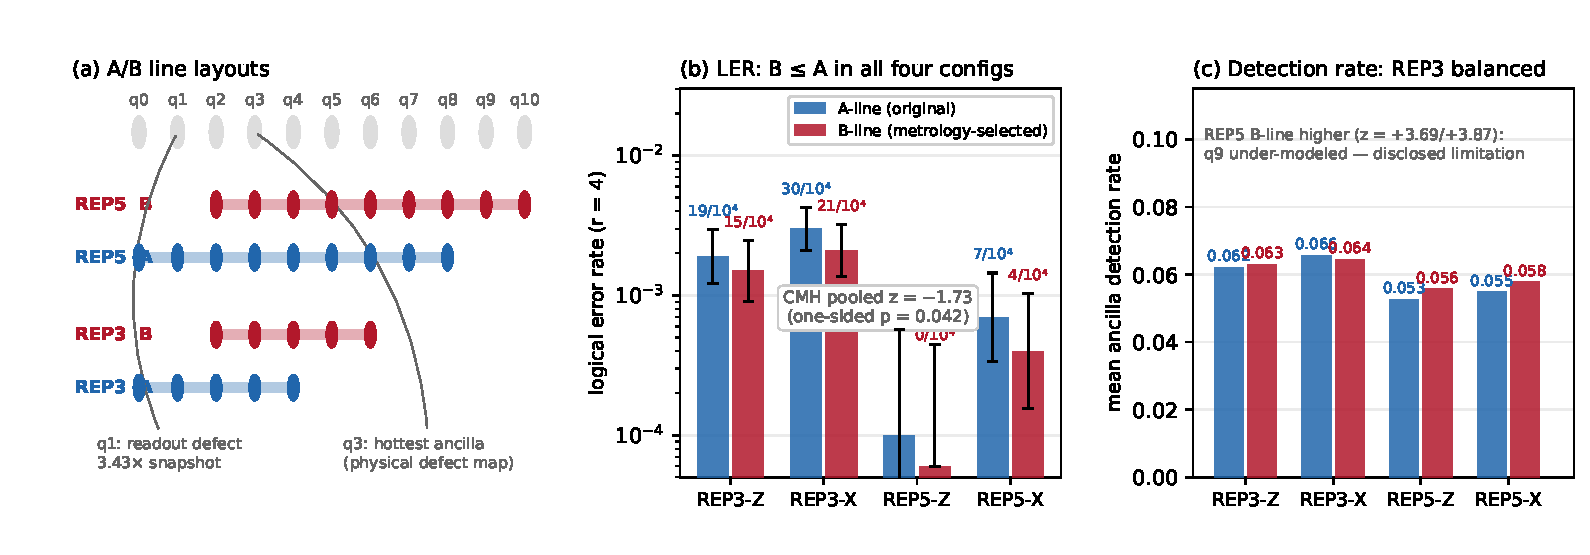
\includegraphics[width=\columnwidth]{figures/ap_f2_ab_result.pdf}
\caption{Active provenance: (a) A/B line layout with defect annotations; (b) logical error rates with Wilson CIs and the CMH pool; (c) per-detector event rates with the REP5 dissociation disclosed.}
\label{fig:ab}
\end{figure}

\section{Pre-registered device test of the injection-budget bound}
\label{app:injection}
%%-----------------------------------------------------------

We test Theorem~\ref{thm:spacetime} and Corollary~\ref{cor:stoch} on ibm\_marrakesh (156-qubit Heron r2) with REP5 ($d{=}5$, $t{=}2$) and REP3 ($d{=}3$, $t{=}1$) memories, both sectors, $R{=}4$ rounds. The adversary injects Pauli faults at round~2 (Z-sector: physical $X$ gates; X-sector: basis-conjugated physical $X$ gates, H-$X$-H, realizing $Z$-type faults on the $\lvert +_L \rangle$ memory; each injected fault is thus implemented with native gates in both sectors). Layouts are the metrology-selected B-lines of Appendix~\ref{app:activeprov}, fixed across all arms so that injection is the only varying factor. Predictions, decision rules, seeds, layouts, and circuit digests were pinned (SHA-256 \texttt{759169c2\dots c74653cd5}) \emph{before} submission; 312 arms (180{,}000 shots) ran in four Sampler jobs (\texttt{da8um21qtnsc73d0v3ug}, \texttt{da8um2ce74ec73aj4n3g}, \texttt{da8um31qtnsc73d0v400}, \texttt{da8um3ke74ec73aj4n50}); the full noiseless pipeline was validated end-to-end (22/22 arms) before submission. $\pi(k)$ entering the composed bounds is estimated from the calibration-snapshot fault model ($\lambda_N{=}0.47$ faults/shot REP5, $0.25$ REP3): $\pi(1..3)=0.375, 0.081, 0.012$ (REP5) and $0.221, 0.027, 0.002$ (REP3). \textbf{Model status of $\pi$:} these tails are predictions of the pinned model. The model uses a Poisson fault-count law with intensity $\lambda_N$ equal to the sum over readout-error locations; gate and idle contributions enter at second order on Heron r2. They are not conservative envelopes over calibration drift; their empirical content is tested by the arms below, not assumed. Scope: this campaign tests the injection-budget bound and the calibration-to-model workflow on repetition memories; it is not a measurement of BB-code hardware performance, and no quantitative REP$\to$BB transfer is claimed.

\begin{table}[htbp]\centering\small
\caption{Deterministic worst-case injection arms (10{,}000 shots each). ``Bound'': Theorem~\ref{thm:spacetime}(c) with calibration $\pi$. A dash indicates that the arm has weight $t+1$, outside its stated range.}
\label{tab:injdet}
\begin{tabular}{@{}llrrrr@{}}
\toprule
arm & sector & failures & LER & bound & verdict \\\midrule
REP5 base & Z & 0 & 0.0000 & 0.012 & holds \\
REP5 base & X & 2 & 0.0002 & 0.012 & holds \\
REP5 $w{=}2$ worst & Z & 414 & 0.0414 & 0.375 & holds \\
REP5 $w{=}2$ worst & X & 506 & 0.0506 & 0.375 & holds \\
REP5 $w{=}3$ worst & Z & 9590 & 0.9590 &--& sharp \\
REP5 $w{=}3$ worst & X & 9598 & 0.9598 &--& sharp \\
REP3 base & Z & 14 & 0.0014 & 0.027 & holds \\
REP3 base & X & 28 & 0.0028 & 0.027 & holds \\
REP3 $w{=}1$ worst & Z & 276 & 0.0276 & 0.221 & holds \\
REP3 $w{=}1$ worst & X & 318 & 0.0318 & 0.221 & holds \\
REP3 $w{=}2$ worst & Z & 9292 & 0.9292 &--& sharp \\
REP3 $w{=}2$ worst & X & 9240 & 0.9240 &--& sharp \\\bottomrule
\end{tabular}
\end{table}

\begin{table}[htbp]\centering\small
\caption{Stochastic injection arms, REP5 (50 pinned variants $\times$ 200 shots per cell). ``Naive (pop.\ avg.)'': the population-averaged independence-form threshold $\delta_0+\Pr[\mathrm{Bin}\ge3]+\mathrm{tol}$. ``Naive (mask-cond.)'': the mask-conditioned estimand, conditioning on the realized pinned masks, $\delta_0+\frac{1}{50}\sum_v\mathbf{1}[w(\mathrm{mask}_v)\ge t{+}1]+\mathrm{tol}$ (\texttt{stoch\_reanalysis.csv}); the verdict is read against this column; the conditioning matches the pinned-mask design of the campaign. Composed: Corollary~\ref{cor:stoch} with calibration $\pi$.}
\label{tab:injstoch}
{\setlength{\tabcolsep}{2.5pt}
\begin{tabular}{@{}llrrrrrl@{}}
\toprule
$p$ & sector & failures & LER & naive (pop.\ avg.) & naive
(mask-cond.) & composed & verdict \\\midrule
0.01 & Z & 1 & 0.0001 & 0.0024 & 0.0024 & 0.016 & holds \\
0.01 & X & 2 & 0.0002 & 0.0027 & 0.0027 & 0.016 & holds \\
0.05 & Z & 6 & 0.0006 & 0.0035 & 0.0024 & 0.035 & holds \\
0.05 & X & 9 & 0.0009 & 0.0039 & 0.0027 & 0.035 & holds \\
0.10 & Z & 211 & 0.0211 & 0.0109 & 0.0224 & 0.070 & holds \\
0.10 & X & 388 & 0.0388 & 0.0113 & 0.0427 & 0.070 & holds \\\bottomrule
\end{tabular}}
\end{table}

Three findings. (i)~\emph{The distance cliff is real and sharp:} weight-$t$ worst-case injections stay within the composed correctability bound on both distances and both sectors, while weight-$(t{+}1)$ injections collapse the memory at $92.4$-$96.0\%$ logical failure; the shortfall from $100\%$ is native-noise rescue of order $\pi(1)$. (ii)~\emph{Injection amplifies native noise exactly as the chain argument predicts:} the REP5 $w{=}2$ arms sit $100$-$250\times$ above baseline but an order of magnitude below the composed bound. This provides a quantitative test of adversary--noise composition for a quantum memory. (iii)~\emph{Stochastic arms: mask-conditioned thresholds.} At $p{=}0.10$ the realized LERs exceed the population-averaged independence-form threshold of Proposition~\ref{prop:stochastic} by $2.1\times$ (Z) and $3.8\times$ (X). The pinned protocol, however, fixes 50 masks per cell, so the appropriate threshold for the pinned ensemble is \emph{mask-conditioned}: the X ensemble realizes two weight-3 masks versus $0.43$ expected under $\mathrm{Bin}(5,0.1)$ (realized tail $0.04$), the Z ensemble one (tail $0.02$). Against the conditioned thresholds ($0.0224$ Z, $0.0427$ X) the realized LERs ($0.0211$, $0.0388$) do \emph{not} exceed, and the same holds for all six cells in both campaigns (\texttt{stoch\_reanalysis.csv}, 12 cells, margins $0.0013$-$0.0039$). The population-average form can undershoot realized-mask risk when the realized ensemble is tail-heavy. This observation motivated the composed Binomial$\otimes$Poisson model (Corollary~\ref{cor:stoch}) and is reported as a discovery rather than a prespecified prediction. The consolidation campaign of Appendix~\ref{app:injection-repl} tests the model under a pre-pinned mask-conditioned estimand. The device-aware composed form holds on all six stochastic arms and all eight bounded deterministic arms under either estimand.

\noindent\textbf{Security corollary.}
Together with the REP5 detection-rate dissociation in Appendix~\ref{app:activeprov}, these results show that syndrome-event statistics alone do not establish the target bound. In the experiments reported here, logical-level injection probes provide direct evidence about $\lambda_{\mathcal{M}}(W)$ under $\mathfrak{A}_1^{\mathrm{st}}(W)$; this does not exclude other valid analytic certification methods.

\subsection{Replication: second calibration cycle, second device, distance~7}\label{app:injection-repl}

A pre-registered consolidation campaign (predictions, decision rules, seeds, layouts, estimator, and digests pinned before submission, SHA-256 \texttt{cef236ce\dots de53aa1}) re-ran the test on ibm\_marrakesh on a second calibration cycle (2026-09-06; 240{,}000 shots in four Sampler jobs \texttt{daelek5nj4cs73afaqpg}, \texttt{daelekd1ierc738mai50}, \texttt{daelel642tqs73auss4g}, \texttt{daeleljdd5gc73d8pcrg}), extended it to REP7 ($d{=}7$, $t{=}3$; worst-case central strings $w{=}3$ and $w{=}4$), and replicated the REP5 deterministic arms on a second device, ibm\_fez (60{,}000 shots; jobs \texttt{daelelt1ierc738mai7g}, \texttt{daelembdd5gc73d8pct0}). Layouts were re-selected from the pinned 2026-09-06 snapshots by the metrology rule of Appendix~\ref{app:activeprov} (the REP5 rule returned the campaign-1 line); the stochastic masks are bit-identical to campaign~1. The native-fault estimator is pinned explicitly, $\lambda_N=\sum_{\mathrm{data}}\epsilon_{\mathrm{ro}}+ R\sum_{\mathrm{anc}}\epsilon_{\mathrm{ro}}$ with symmetric readout $\epsilon_{\mathrm{ro}}$ (readout locations dominate the Heron-r2 spacetime budget; gate/idle terms are second order): $\lambda_N{=}0.088, 0.222, 0.347$ (REP3/5/7, marrakesh) and $0.453$ (REP5, fez); the 2026-09-06 marrakesh calibration is substantially cleaner than that of 2026-08-28 ($\lambda_N{=}0.25, 0.47$). Noiseless end-to-end validation passed on all 42 checked arms before submission.

\begin{table}[htbp]\centering\small
\caption{Consolidation deterministic arms (10{,}000 shots each): REP7 extension (ibm\_marrakesh) and second-device REP5 replication (ibm\_fez). ``Bound'': Theorem~\ref{thm:spacetime}(c) with the pinned calibration $\pi$. A dash indicates that the arm has weight $t+1$, outside its stated range.}
\label{tab:injrepl}
\begin{tabular}{@{}lllrrrl@{}}
\toprule
device & arm & sector & failures & LER & bound & verdict \\\midrule
marrakesh & REP7 base & Z & 0 & 0.0000 & 0.0005 & holds \\
 & REP7 $w{=}3$ worst & Z & 568 & 0.0568 & 0.293 & holds \\
 & REP7 $w{=}4$ worst & Z & 9691 & 0.9691 &--& sharp \\
 & REP7 base & X & 1 & 0.0001 & 0.0005 & holds \\
 & REP7 $w{=}3$ worst & X & 675 & 0.0675 & 0.293 & holds \\
 & REP7 $w{=}4$ worst & X & 9599 & 0.9599 &--& sharp \\\midrule
fez & REP5 base & Z & 1 & 0.0001 & 0.011 & holds \\
 & REP5 $w{=}2$ worst & Z & 484 & 0.0484 & 0.364 & holds \\
 & REP5 $w{=}3$ worst & Z & 9768 & 0.9768 &--& sharp \\
 & REP5 base & X & 6 & 0.0006 & 0.011 & holds \\
 & REP5 $w{=}2$ worst & X & 683 & 0.0683 & 0.364 & holds \\
 & REP5 $w{=}3$ worst & X & 9745 & 0.9745 &--& sharp \\\bottomrule
\end{tabular}
\end{table}

Four findings. (i)~\emph{Full replication.} On the new calibration cycle every campaign-1 verdict reproduces: all bounded deterministic arms sit $4$-$8\times$ inside the composed bound on both distances and sectors (REP3 $w{=}1$: $0.0102/0.0202$ vs bound $0.084$; REP5 $w{=}2$: $0.0333/0.0436$ vs $0.199$), all weight-$(t{+}1)$ arms remain sharp ($0.898$-$0.974$), and all six stochastic cells track campaign~1 within statistical noise (at $p{=}0.10$: $0.0202$ vs $0.0211$ Z; $0.0403$ vs $0.0388$ X). The campaign-1 excess over the population-averaged independence-form threshold replicates ($1.9\times$ Z, $3.6\times$ X), and, as in campaign~1, no cell exceeds the mask-conditioned threshold ($0.0224$ Z, $0.0426$ X); for this consolidation the estimand was part of the pre-submission pinning, so no falsification occurs in either campaign under the mask-conditioned estimand (\texttt{stoch\_reanalysis.csv}). (ii)~\emph{The cliff has a third distance point.} REP7 behaves as Theorem~\ref{thm:spacetime} demands: weight-$3$ worst-case injections stay inside the bound ($0.057/0.068$ vs $0.293$) while weight-$4$ collapses the memory at $96.0$-$96.9\%$; the cliff is sharp at $d{=}3,5,7$. (iii)~\emph{Cross-device.} The REP5 pattern reproduces on ibm\_fez with its own pinned calibration ($\lambda_N{=}0.453$): bounds hold at $5$-$7\times$ margin, sharpness at $97.5$-$97.7\%$. (iv)~\emph{Mask-level composition.} With the cleaner calibration the population-average binomial-form composed bound tightens ($0.0335$ for the X-sector $p{=}0.10$ cell), and the realized LER ($0.0403$) exceeds that population-average form by $1.20\times$; the excess is accounted for by the realized pinned-mask ensemble. The X masks contain two weight-3 variants, compared with $0.43$ expected under $\mathrm{Bin}(5,0.1)$; these variants contribute $0.0375$. Conditioning the composed bound on the realized masks (bound $0.0665$) restores the bound, consistent with composition holding mask-by-mask rather than only in binomial expectation. This is the same estimand correction as in campaign~1, applied to the composed model. Absolute LERs of bounded arms drift down coherently with the cleaner calibration ($\lambda_N$: $0.47{\to}0.22$), while cliff arms drift slightly up (less native-noise rescue of order $\pi(1)$), exactly as the model predicts. The consolidation artifacts (\texttt{theory\_test\_consol/}) are archived with the same digest discipline as campaign~1.

%%----------------------------------------------------------
\section{Illustrative routing arithmetic}\label{app:routing}
\emph{Heuristic only; LFR underestimates diamond-norm error.} $J=8$, $b=1$, $\Delta=0.05$: $p_\mathrm{hit}\le0.175$. CZ at $p=5\times10^{-4}$: $(0.825)(0.905)=0.747$. MS: $(0.825)(0.955)=0.788$.


\bibliography{references}

\end{document}
